\documentclass[a4paper,12pt]{report}

\usepackage{alltt, fancyvrb, url}
\usepackage{graphicx}
\usepackage[utf8]{inputenc}
\usepackage{float}
\usepackage{xcolor}
\usepackage{hyperref}

\usepackage[italian]{babel}

\usepackage[italian]{cleveref}

\title{OOP24 - RUNWARRIOR}
\author{
    Samuele Bianchedi, Riccardo Cornacchia\\
    Francesca Gatti, Giovanni Maria Rava}
\date{\today}
\begin{document}
\maketitle
\tableofcontents
\chapter{Analisi}
\section{Descrizione e requisiti}
Il gruppo si pone come obbiettivo quello di realizzare una reinterpretazione del famoso gioco 
Super Mario Bross del 1986. Il gioco ha come personaggio principale un cavaliere, che tramite 
l'input dell'utente si muove in una mappa 2D. L'obbiettivo del cavaliere è salvare una princessa tenuta
prigioniera da uno stregone, completando diversi livelli che lo condurranno al castello nel quale è 
rinchiusa. Nel gioco sarà possibile, tramite un negozio, comprare un altro personaggio, se si ha raccolto un numero sufficiente di monete.
All'interno del gioco, oltre a diversi ostacoli, sono presenti nemici che il cavaliere può uccidere per rimanere in vita e 
completare il livello. 
\subsection*{Requisiti funzionali}
\begin{itemize}
    \item Il personaggio deve avanzare, indietreggiare e saltare all'interno della mappa.
    \item Gestione delle collisioni del personaggio con nemici, ostacoli, monete e potenziamenti.
    \item Il personaggio può ottenere due potenziamenti che lo aiuteranno nella sua avventura.
    \item Gestione di nemici ed ostacoli diversi in base alla mappa.
    \item Creazione di un sistema di punteggio, che verrà mostrato al completamento del livello.
\end{itemize}
\newpage
\subsection*{Requisiti non funzionali}
\begin{itemize}
    \item Implementazioni di una quarta mappa. 
    \item Gestione di restart e checkpoint.
    \item Creazione di nemici e ostacoli più complessi.
    \item Musica e suoni. 
\end{itemize}
\section{Modello del Dominio}
RunWarrior è gioco ambientato in un mondo fantastico in cui il personaggio principale deve affrontare 3 livelli diversi, selezionabili mediante un menù.
In questi livelli il personaggio deve portersi muovere per sopravvivere e uccidere i nemici. Il movimento del personaggio è gestito tramite tastiera.
All'interno della mappa sono posizionate delle uova che racchiudono al loro interno i 2 possibili powerup, diversi per Warrior e Wizard.
Per il completamento del gioco è neccessario sbloccare tutti i livelli in maniera sequenziale, che si considerano terminati 
tramite l'ingresso in un portale, ad eccezione del terzo che si conclude con il castello della principessa.
All'interno di ogni livello possono essere presenti degli ostacoli letali (MapElement) e dei nemici (Enemy) e delle monete (Coin) con il quale il 
personaggio può collidere. Se ciò accade con un ostacolo o con un nemico perde un potenziamento, nel caso lo avesse, altrimenti la partita finisce.
I nemici sono di 5 tipi:
\begin{itemize}
    \item Goblin
    \item Snake
    \item Wizard
    \item Monkey 
    \item Guard
\end{itemize}
Gli ostacoli letali sono:
\begin{itemize}
    \item Fungo
    \item Cactus
    \item Camino con fuoco
\end{itemize}

\begin{figure}
    \centering
    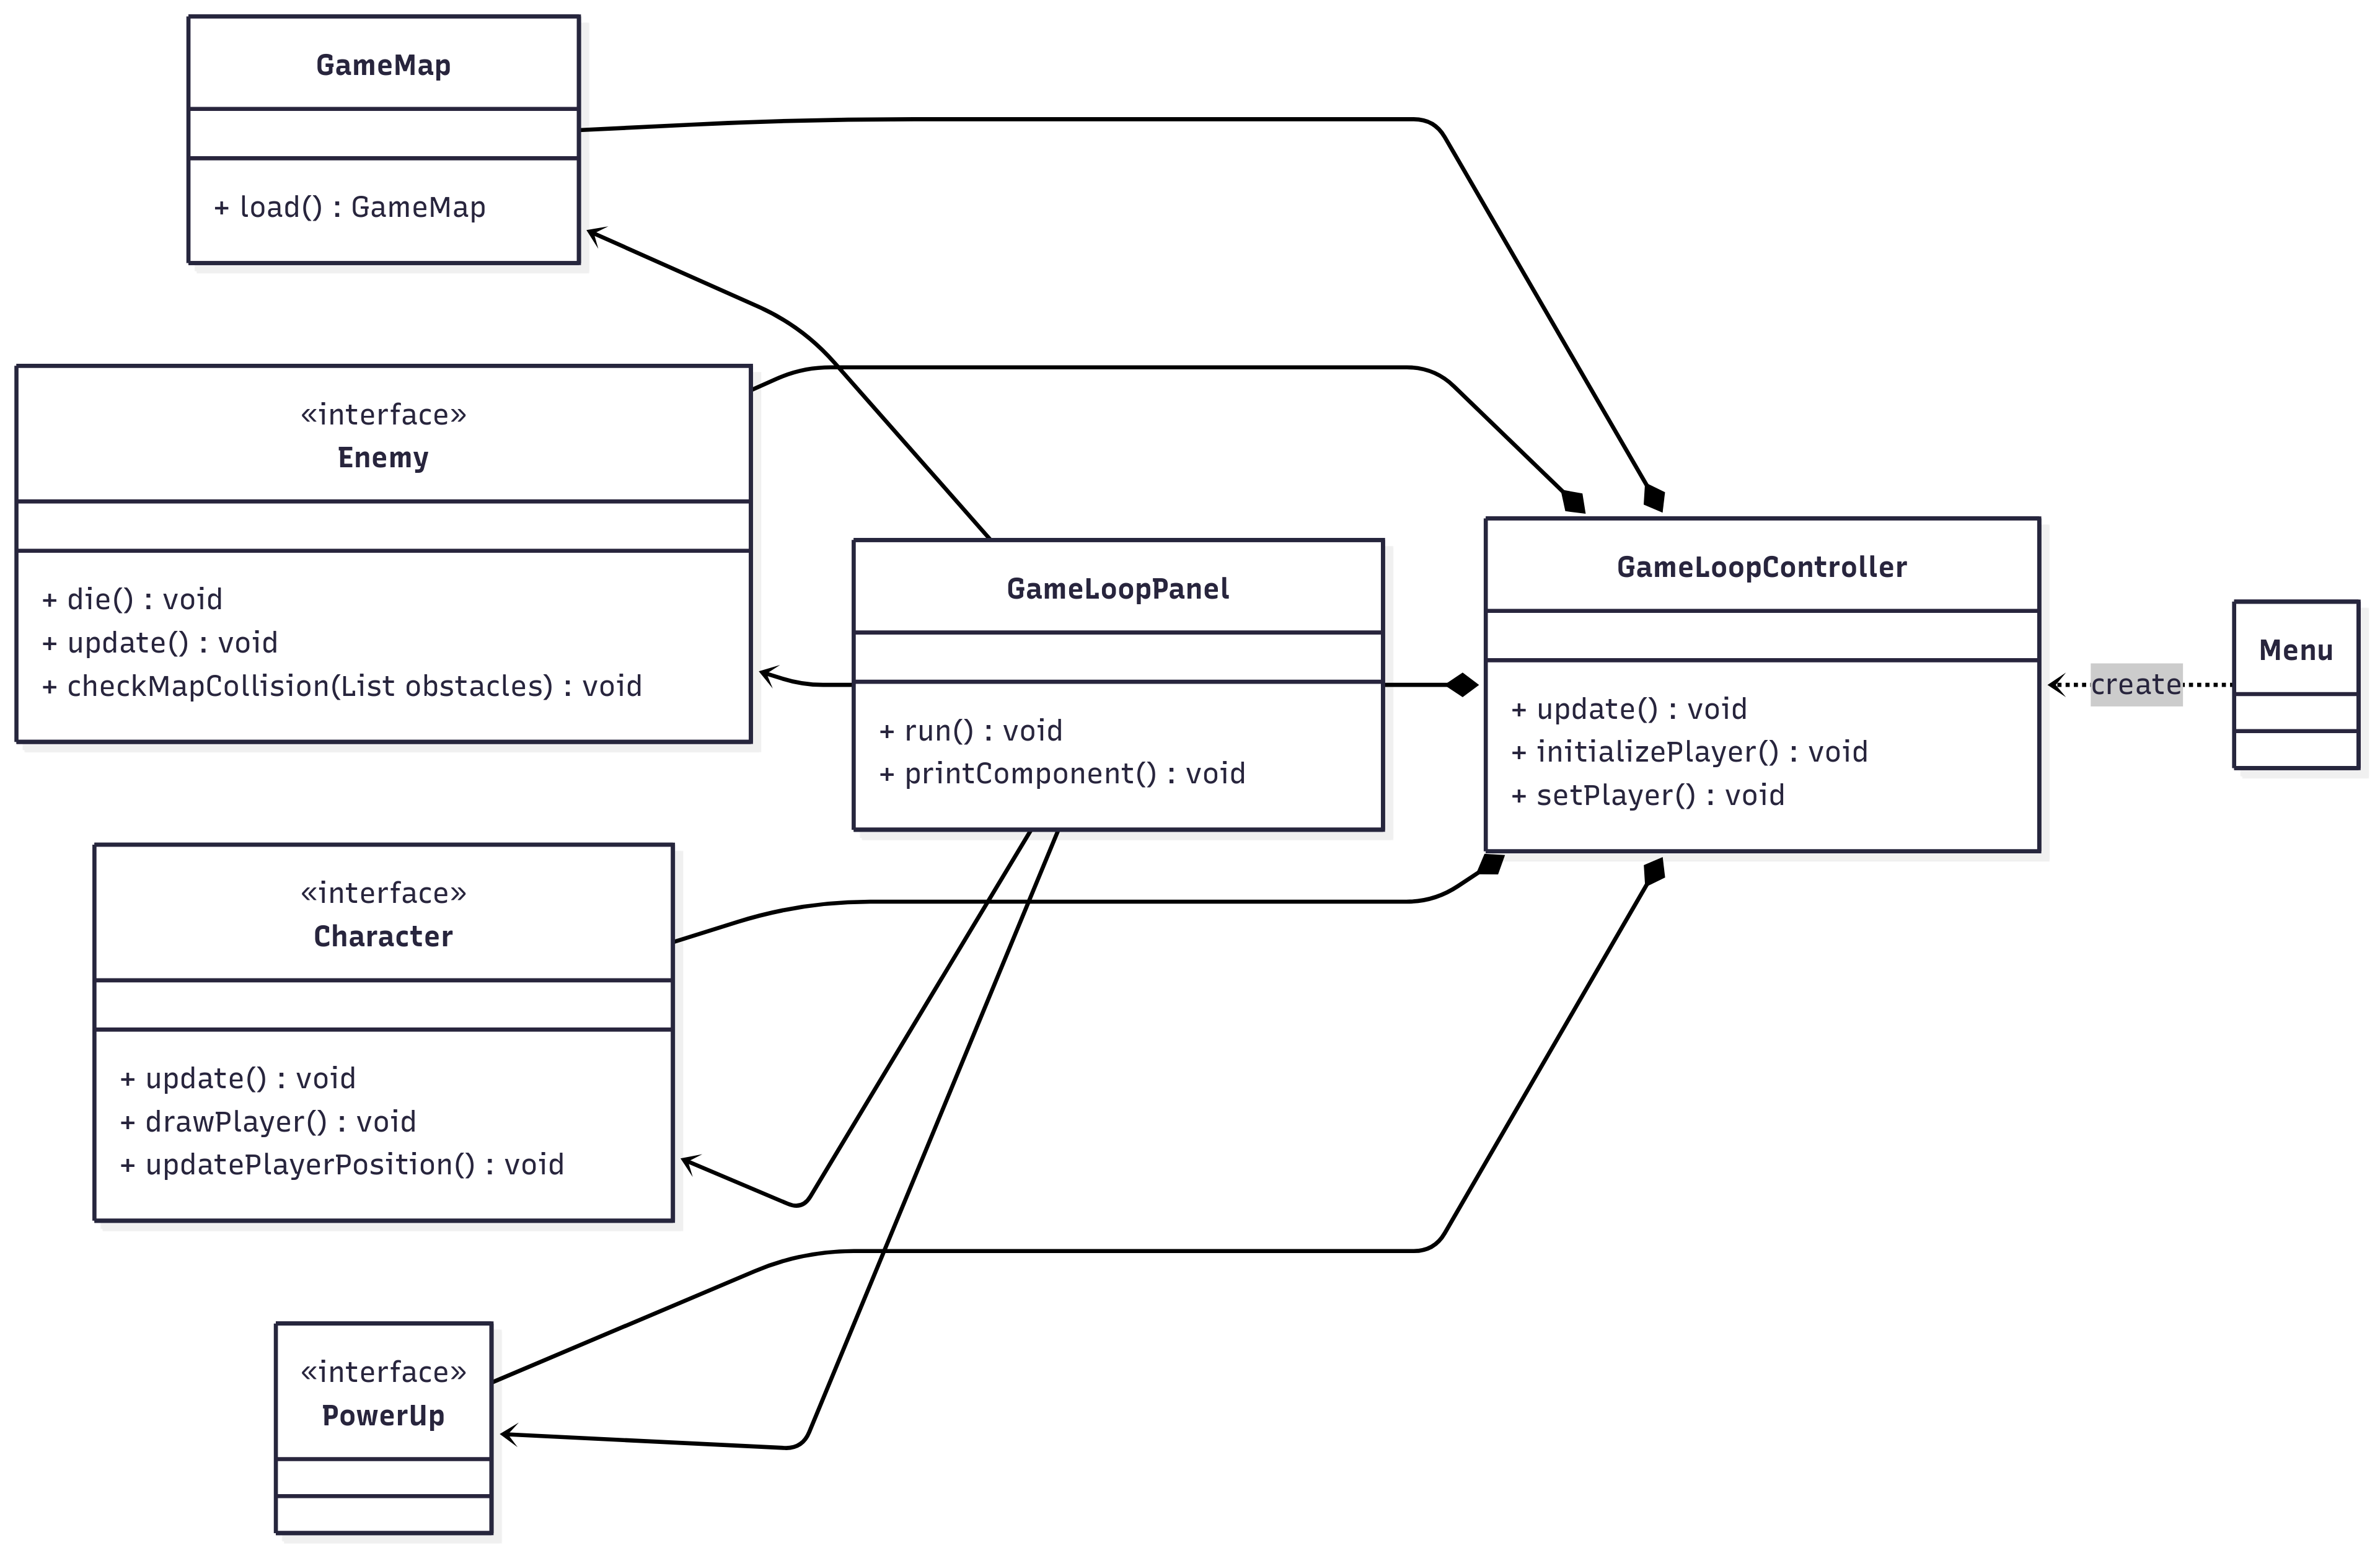
\includegraphics[width=\textwidth]{resources/modelloDominioUML.png}
    \caption{UML del modello del dominio}
    \label{}
\end{figure}
\chapter{Design}
\section{Architettura}
L'architettura di RunWarrior segue il pattern architetturale MVC (Model - View - Controller). Il GameLoopController gestisce l'aggiornamento
del gioco e di tutte le sue entità a seguito dei diversi eventi che possono capitare durante la sessione. All'interno della classe, 
dal momento in cui viene acquistato il nuovo personaggio, ricevendo le informazione da GameSaveManager e Shop, viene gestito il cambio skin.
Gli input da tastiera per muovere il personaggio vengono gestiti tramite la comunicazione tra le classi CharacterComand e MovementHandlerImpl.
Quindi il Character è una entità reattiva che modifica il proprio stato a seguito delle diverse collisioni con le diverse entità.
Il pattern MVC implementato consente di mantenere lo stato del controller nell'eventualità che si modifichi la view.
inserire UML delle classi principali dell'MVC
\section{Samuele Bianchedi}
\textbf{Problema}: L'implementazioni delle classi del modello soffriva di una criticità legata all'incapsulamento. SptoBugs ha rilevato molti warning che indicavano oggetti mutabili passati e restituiti tramite riferimento diretto.
Questo poteva creare un'architettura fragile, incline ad errori e/o modifiche involontarie.
\textbf{Soluzione}: Per risolvere questo problema e rendere sicuro i dati ho scelto di implementare copie difensive.
\begin{itemize}
    \item Per oggetti come BufferedImage e int[][]: nei costruttori e nei metodi setter invece di memorizzare il riferimento all'oggetto, 
    ne viene creata una copia completa.
    \item Nei metodi getter: invece di restituire una riferimento all'oggetti ne viene creato uno nuovo da passare al chiamante
    \item Per le collezioni: i metodi getter sono stati modificato per restituire una vista immodificabile della collezione.
\end{itemize}
I pro sono ovviamente la sicurezza dei dati che sono protetti da modifiche esterne. Di contro abbiamo una riduzione della performance, 
in quanto copiare oggetti innumerevoli volte costa abbastanza e in alcuni casi ha portato a “freeze” dell'applicazione.
Nel seguente schema UML si mostra come i campi siano privati e l'accesso avvenga tramite metodi pubblici che lavorano restituendo copie.
\begin{figure}
    \centering
    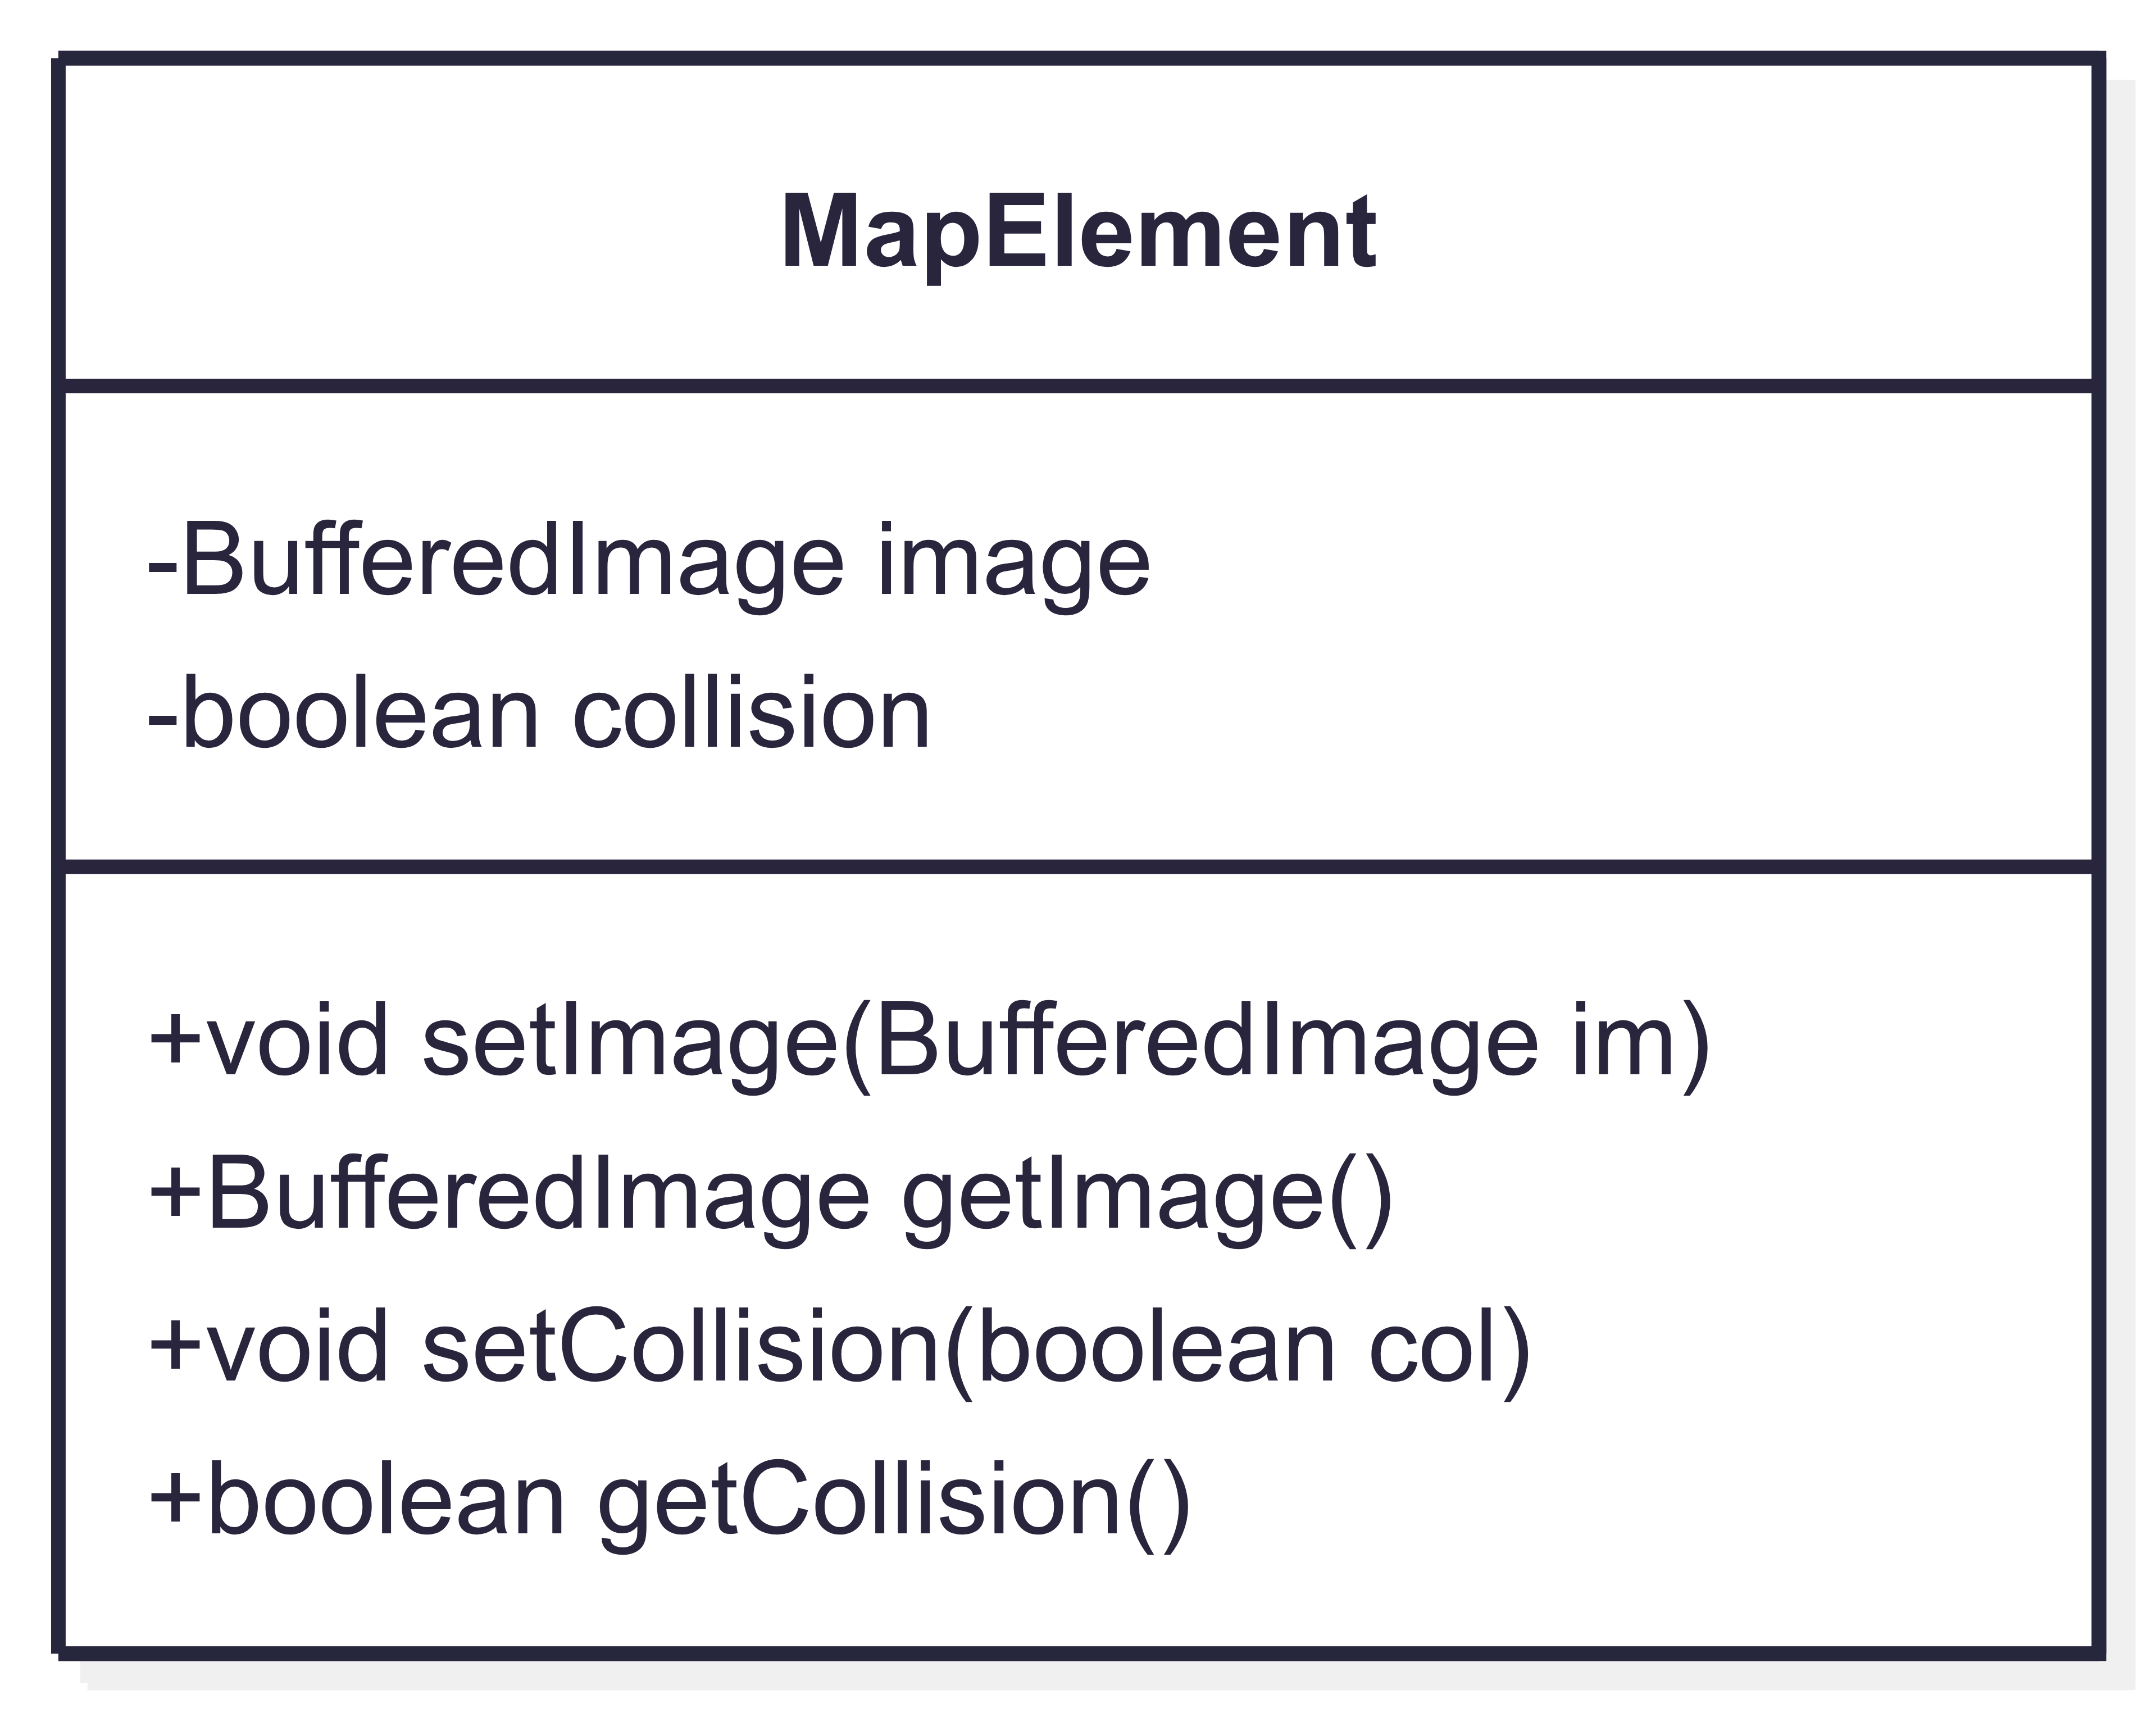
\includegraphics[width=0.8\textwidth]{resources/UMLMapElement.png}
    \caption{UML della classe MapElement nel model}
    \label{}
\end{figure}
Il pattern utilizzato è stato Immutable Object, un idioma fondamentale di OOP. Quest'ultimo spiega gli oggetti immutabili, oggetti che non
si possono veder modificato lo stato dopo la loro creazione. Sebbene gli oggetti nel progetto non siano perfettamente immutabili a causa
dei setter, quello a cui si aspirava era un oggetto non modificabile lontano da errori imprevedibili.
\section{Riccardo Cornacchia}

\textbf{Problema}: si deve gestire la creazione del player considerando che le 2 entità warrior e wizard possono cambiare in modo attivo 3 skin
(senza armatura, con armatura, con armatura e spada/bastone) durante la sessione di gioco.\vspace{1cm}

\textbf{Soluzione}: all'interno dell'architettura MVC, ho realizzato una classe astratta AbstractCharacterImpl che implementa l'interfaccia 
Character per creare l'entità player, nel model del progetto. In questa classe vengono definiti metodi standard che il player esegue sempre 
e i campi che ogni entità player deve avere.

Tale classe astratta viene estesa da 6 classi concrete (NakedWarrior, NakedWizard, ArmourWarrior, ArmourWizard, SwordWarrior, 
StickWizard). Ogni sottoclasse fa Override del metodo astratto playerImage(), per settare le immagini corrispondenti alla skin 
attualmente in gioco, mentre SwordWarrior e StickWizard fanno Override del metodo updateAttackCollision() che setta l'eventuale area dell'arma.
AbstractCharacterImpl implementa il metodo update(), che richiama i 2 metodi modificati ad hoc da ciascuna sottoclasse.

Tramite questa architettura viene sfruttato il Template pattern che stabilisce lo scheletro dell'operazione 
principale (update) nella classe astratta e delega alle sottoclassi la definizione di uno o più aspetti specifici dell'algoritmo 
(playerImage e updateAttackCollision). Il Template method è l'update() che definisce l'algoritmo principale; esso infatti richiama i due 
metodi definiti dalle sottoclassi.

\begin{figure}
    \centering
    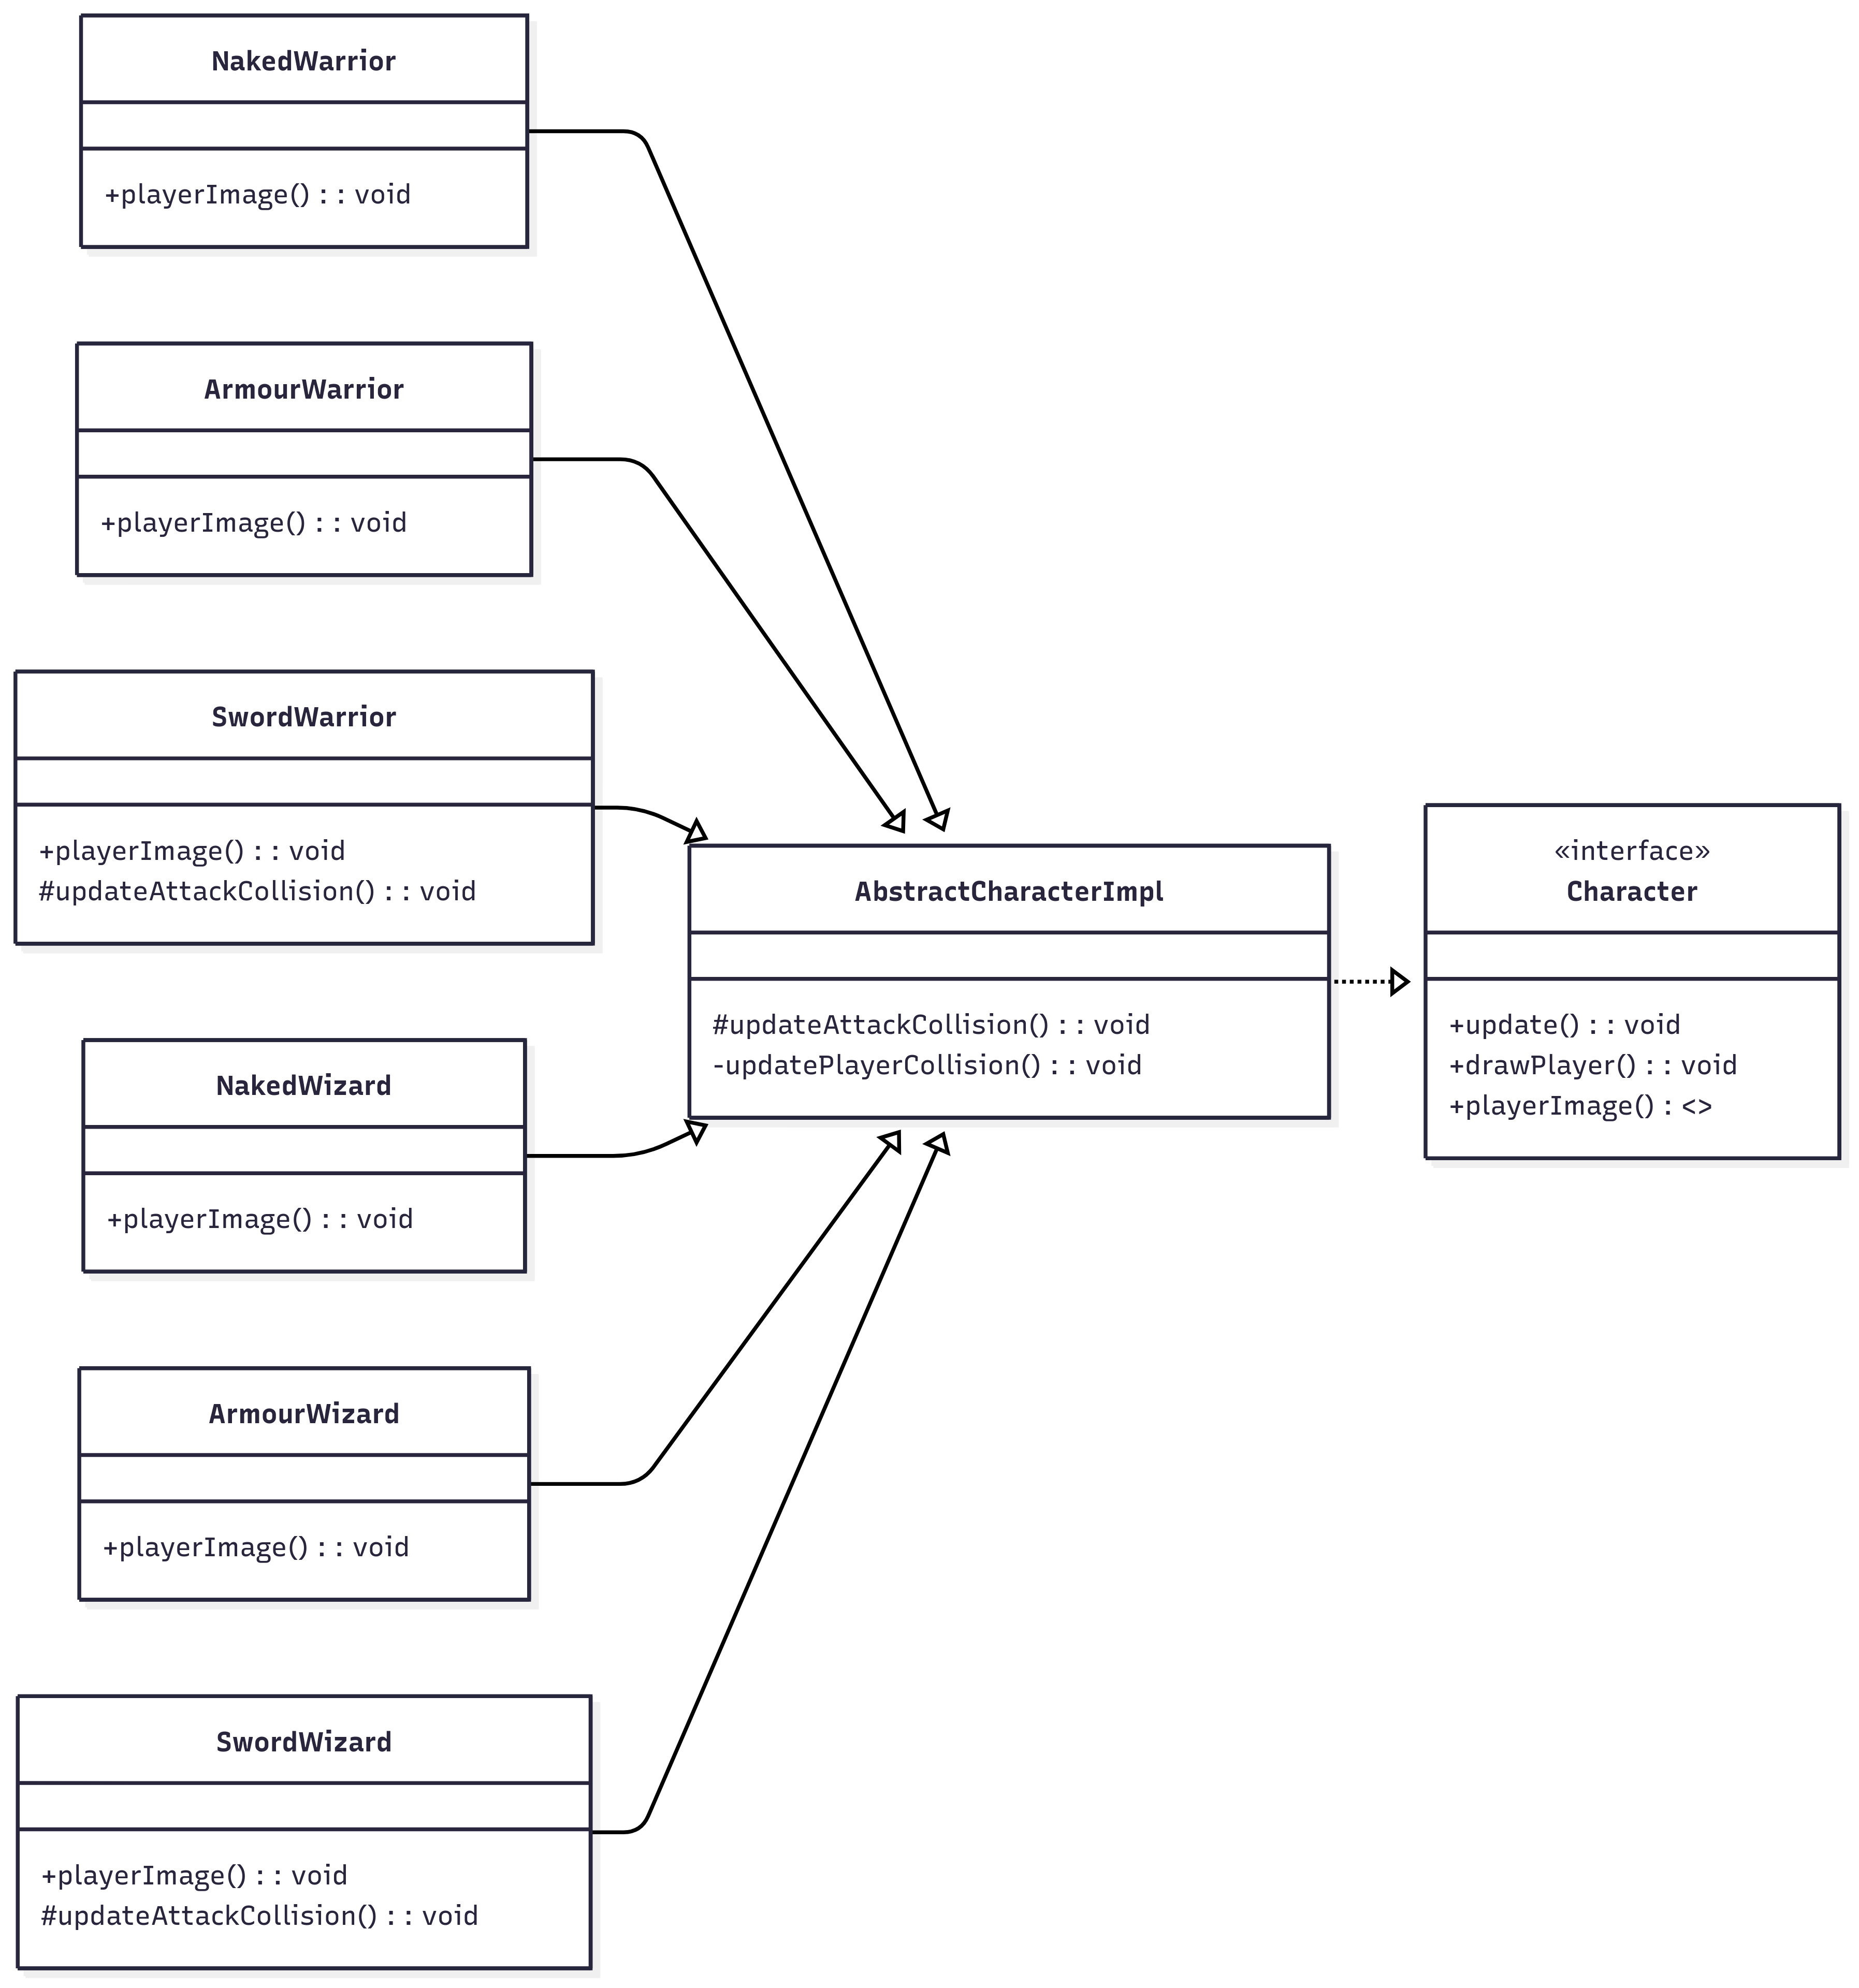
\includegraphics[width=0.8\textwidth]{resources/TemplateCharacter.png}
    \caption{UML del pattern Template per il personaggio principale}
    \label{fig:2.1}
\end{figure}


\textbf{Problema}: gestione dell'animazione, ovvero il cambio continuo dei frame per ogni specifica azione del personaggio; 
gestione del movimento del player, collegato ad input da tastiera.\vspace{1cm}

\textbf{Soluzione}: all'interno dell'architettura MVC , ho realizzato due interfacce CharacterAnimationHandler e 
CharacterMovementHandler, rispettivamente implementate da CharacterAnimationHandlerImpl e CharacterMovementHandlerImpl, nel controller 
del progetto. L'obbiettivo è quello di delegare i 2 comportamenti fondamentali di ogni entità player a due classi distinte nella sezione 
controller.

Entrambe le interfacce vengono usate da AbstractCharacterImpl e i loro metodi vengono richiamati all'interno di update() 
e drawPlayer(Graphics2D).
Per questa architettura mi sono basato sul pattern Strategy, ma applicandone una variazione, cioè incapsulare in 2 interfacce diverse 
le operazioni che gestiscono animazione e movimento del player. Queste due interfacce rappresentano la strategia. Per gestire 
tali comportamenti, entrambe le classi usano CharacterComand, la classe che gestisce l'input da tastiera.

CharacterAnimationHandler definisce metodi fondamentali come: frameChanger(), per gestire il cambiamento dei frame in base agli input 
e imagePlayer(boolean rightDirection), che fornisce l'immagine corretta in base al frame corrente.
CharacterMovementHandler definisce metodi fondamentali come: setLocationAfterPowerUp(), per reimpostare la posizione del player
dopo aver guadagnato o perso una vita e movePlayer(), per gestire spostamento a destra e sinistra, salto e collisione con le diverse 
entità.

\begin{figure}[H]
    \centering
    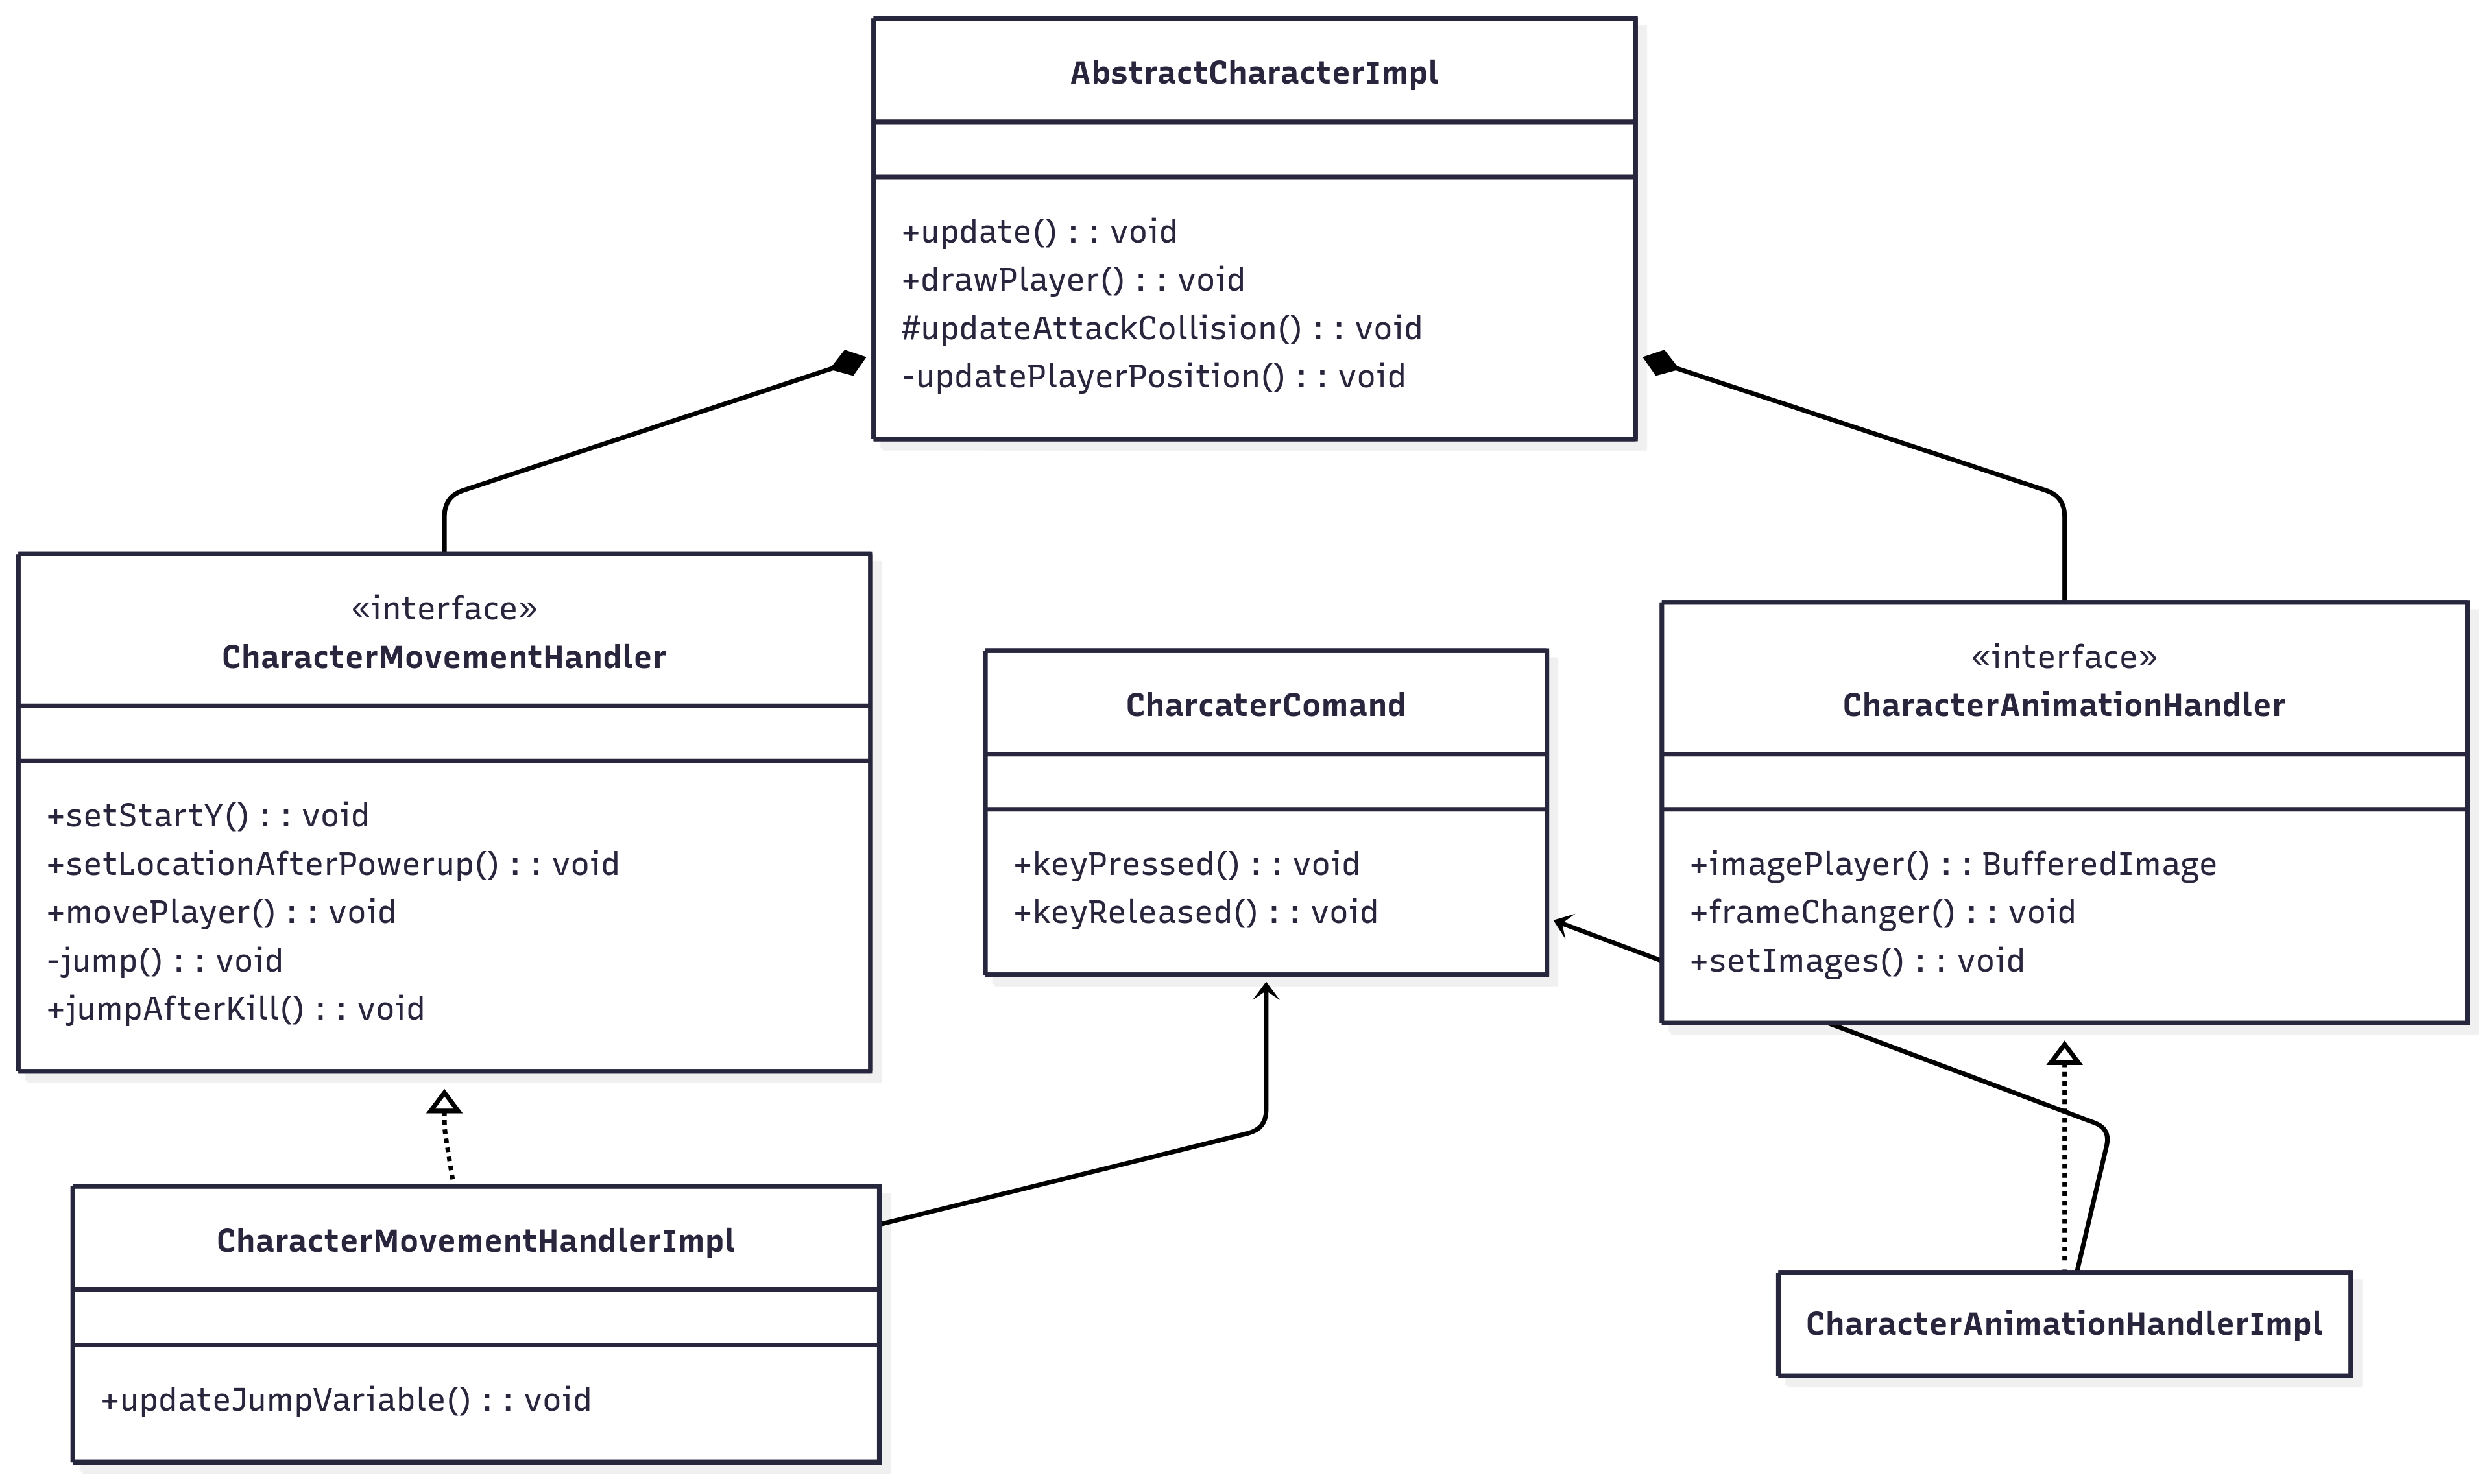
\includegraphics[width=0.8\textwidth]{resources/playerAction.png}
    \caption{UML architettura implementazione animazione e movimento player}
    \label{fig:2.2}
\end{figure}


\textbf{Problema}: gestione delle collisioni con le diverse entità: blocchi della mappa, powerups, nemici e monete. 
Mantenere la relazione con le classi che gestiscono eventuali conseguenze di una specifica collisione.\vspace{1cm}

\textbf{Soluzione}: in questo caso all'interno dell'architettura MVC , ho realizzato quattro interfacce nel controller del progetto, 
ognuna delle quali gestisce le collisioni con 1 delle quattro entità: CollisionDetection, per i blocchi delle mappe, PowerUpDetection, 
per la collisione con l'uovo e i powerups, KillDetection, per i nemici, e CoinDetection, per le monete, 
rispettivamente implementate da CollisionDetectionImpl, PowerUpDetectionImpl, KillDetectionImpl e CoinDetectionImpl.

Le quattro interfacce vengono usate da CharacterMovementHandlerImpl e i loro metodi vengono richiamati all'interno di movePlayer().
Le quattro interfacce descritte rappresentano la strategia per il pattern Strategy, che anche in questo caso non si tratta di Strategy puro, 
ma di una definizione di quattro strategie separate, infatti ognuna di esse incapsula i metodi utili a verificare le collisioni con le 
diverse entità.

\begin{itemize}
    \item CollisionDetection usa checkCollision(), che verifica la collisione del player con i blocchi della mappa tenendo conto di 6 punti 
    della sua area di collisione che lo "circonda". Per verificare che tipologia di blocco viene toccata e in quale direzione avviene
    la collisione richiama touchSolid() e checkCollisionDirection().
    Inoltre fornisce i metodi gameOver() e win() che restituiscono true se il player muore o arriva al portale.
    \item PowerUpDetection usa checkCollisionWithPowers(), che permette al player di bloccarsi se collide con l'uovo, o di raccogliere un 
    powerup quando l'uovo è stato aperto; tutto ciò avviene consultando la lista di powerups creata dal PowerUpController.
    \item KillDetection usa checkCollisionWithEnemies(), che permette di identificare 2 tipi di collisione: se il player schiaccia il nemico, 
    lo uccide, se viene toccato da destra o sinistra perde una vita. La posizione dei nemici viene controllata in loop mediante 
    la lista creata da EnemyHandlerImpl.
    \item CoinDetection usa controlCoinCollision(), che scorre la lista di monete creata da CoinController e quando l'area del player collide 
    con l'area di una moneta viene aggiornato il conteggio delle monete.
\end{itemize}

\begin{figure}[H]
    \centering
    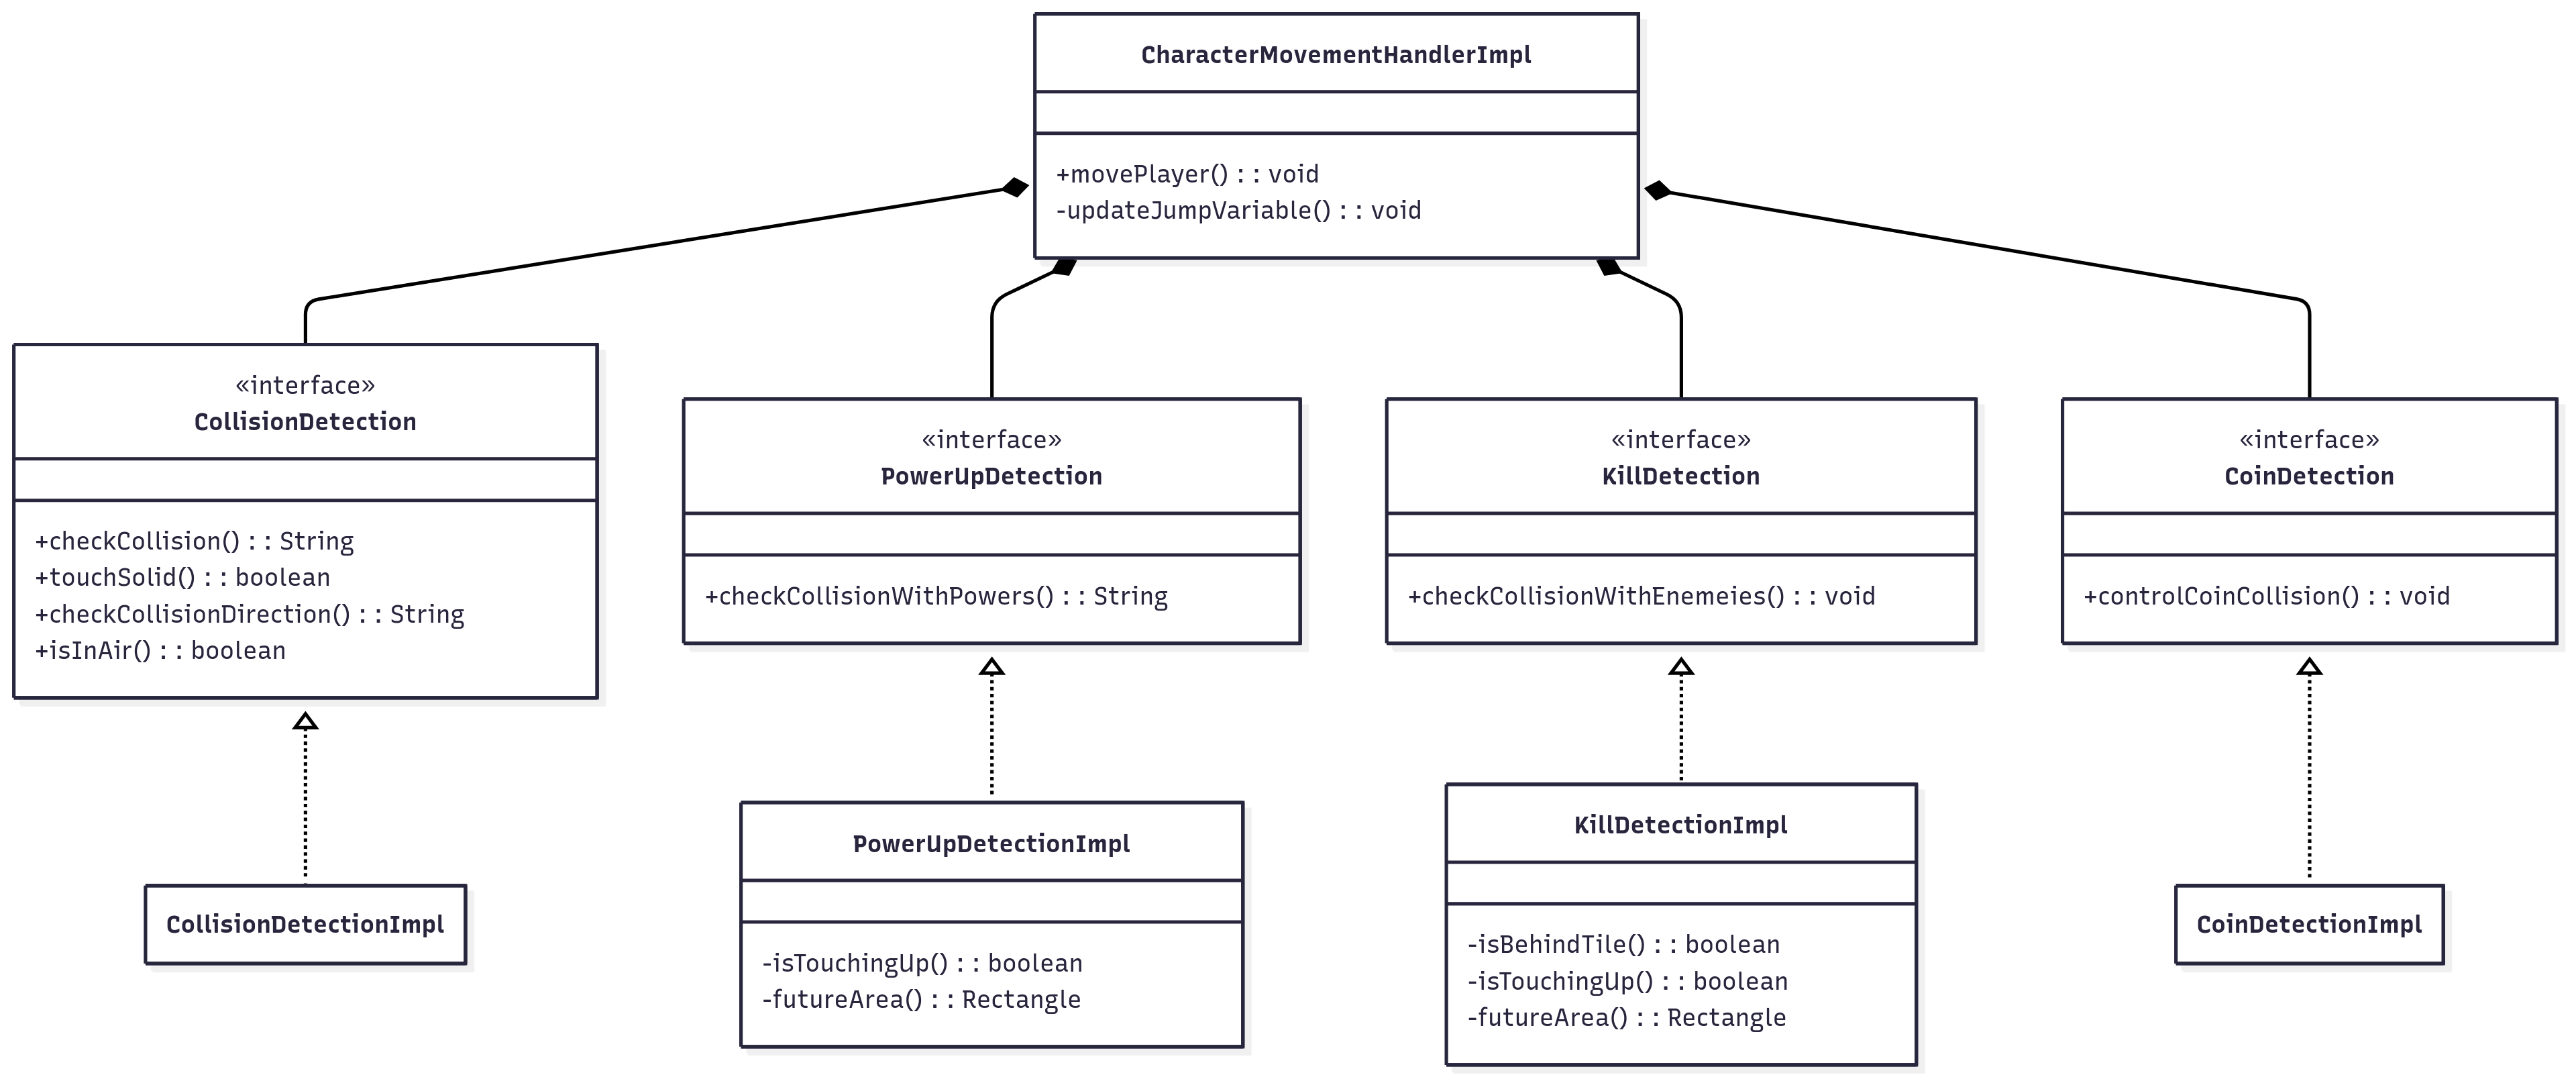
\includegraphics[width=0.8\textwidth]{resources/Collisions.png}
    \caption{UML architettura per gestire le collisioni}
    \label{fig:2.3}
\end{figure}

\textbf{Problema}: creazione dell'entità powerup con meccanica complessa (raccolta powerup solo dopo apertura uovo) e gestione 
delle collisioni col player.\vspace{1cm}

\textbf{Soluzione}: in questo caso ho sfruttato il pattern architetturale MVC creando l'interfaccia PowerUp che realizza l'entità powerup 
e la sua implementazione PowerUpImpl nel model del progetto. Nel controller del progetto ho creato la classe PowerUpController 
con lo scopo di creare la lista dei powerups presenti nelle varie mappe. Infine nella view ho inserito la classe PowerUpManager, 
che acquisisce la lista di tutti i powerups e si occupa di stamparli a video nel pannello di gioco. La collsione tra player e lista 
di powerup è gestita da PowerUpDetection.

\begin{figure}[H]
    \centering
    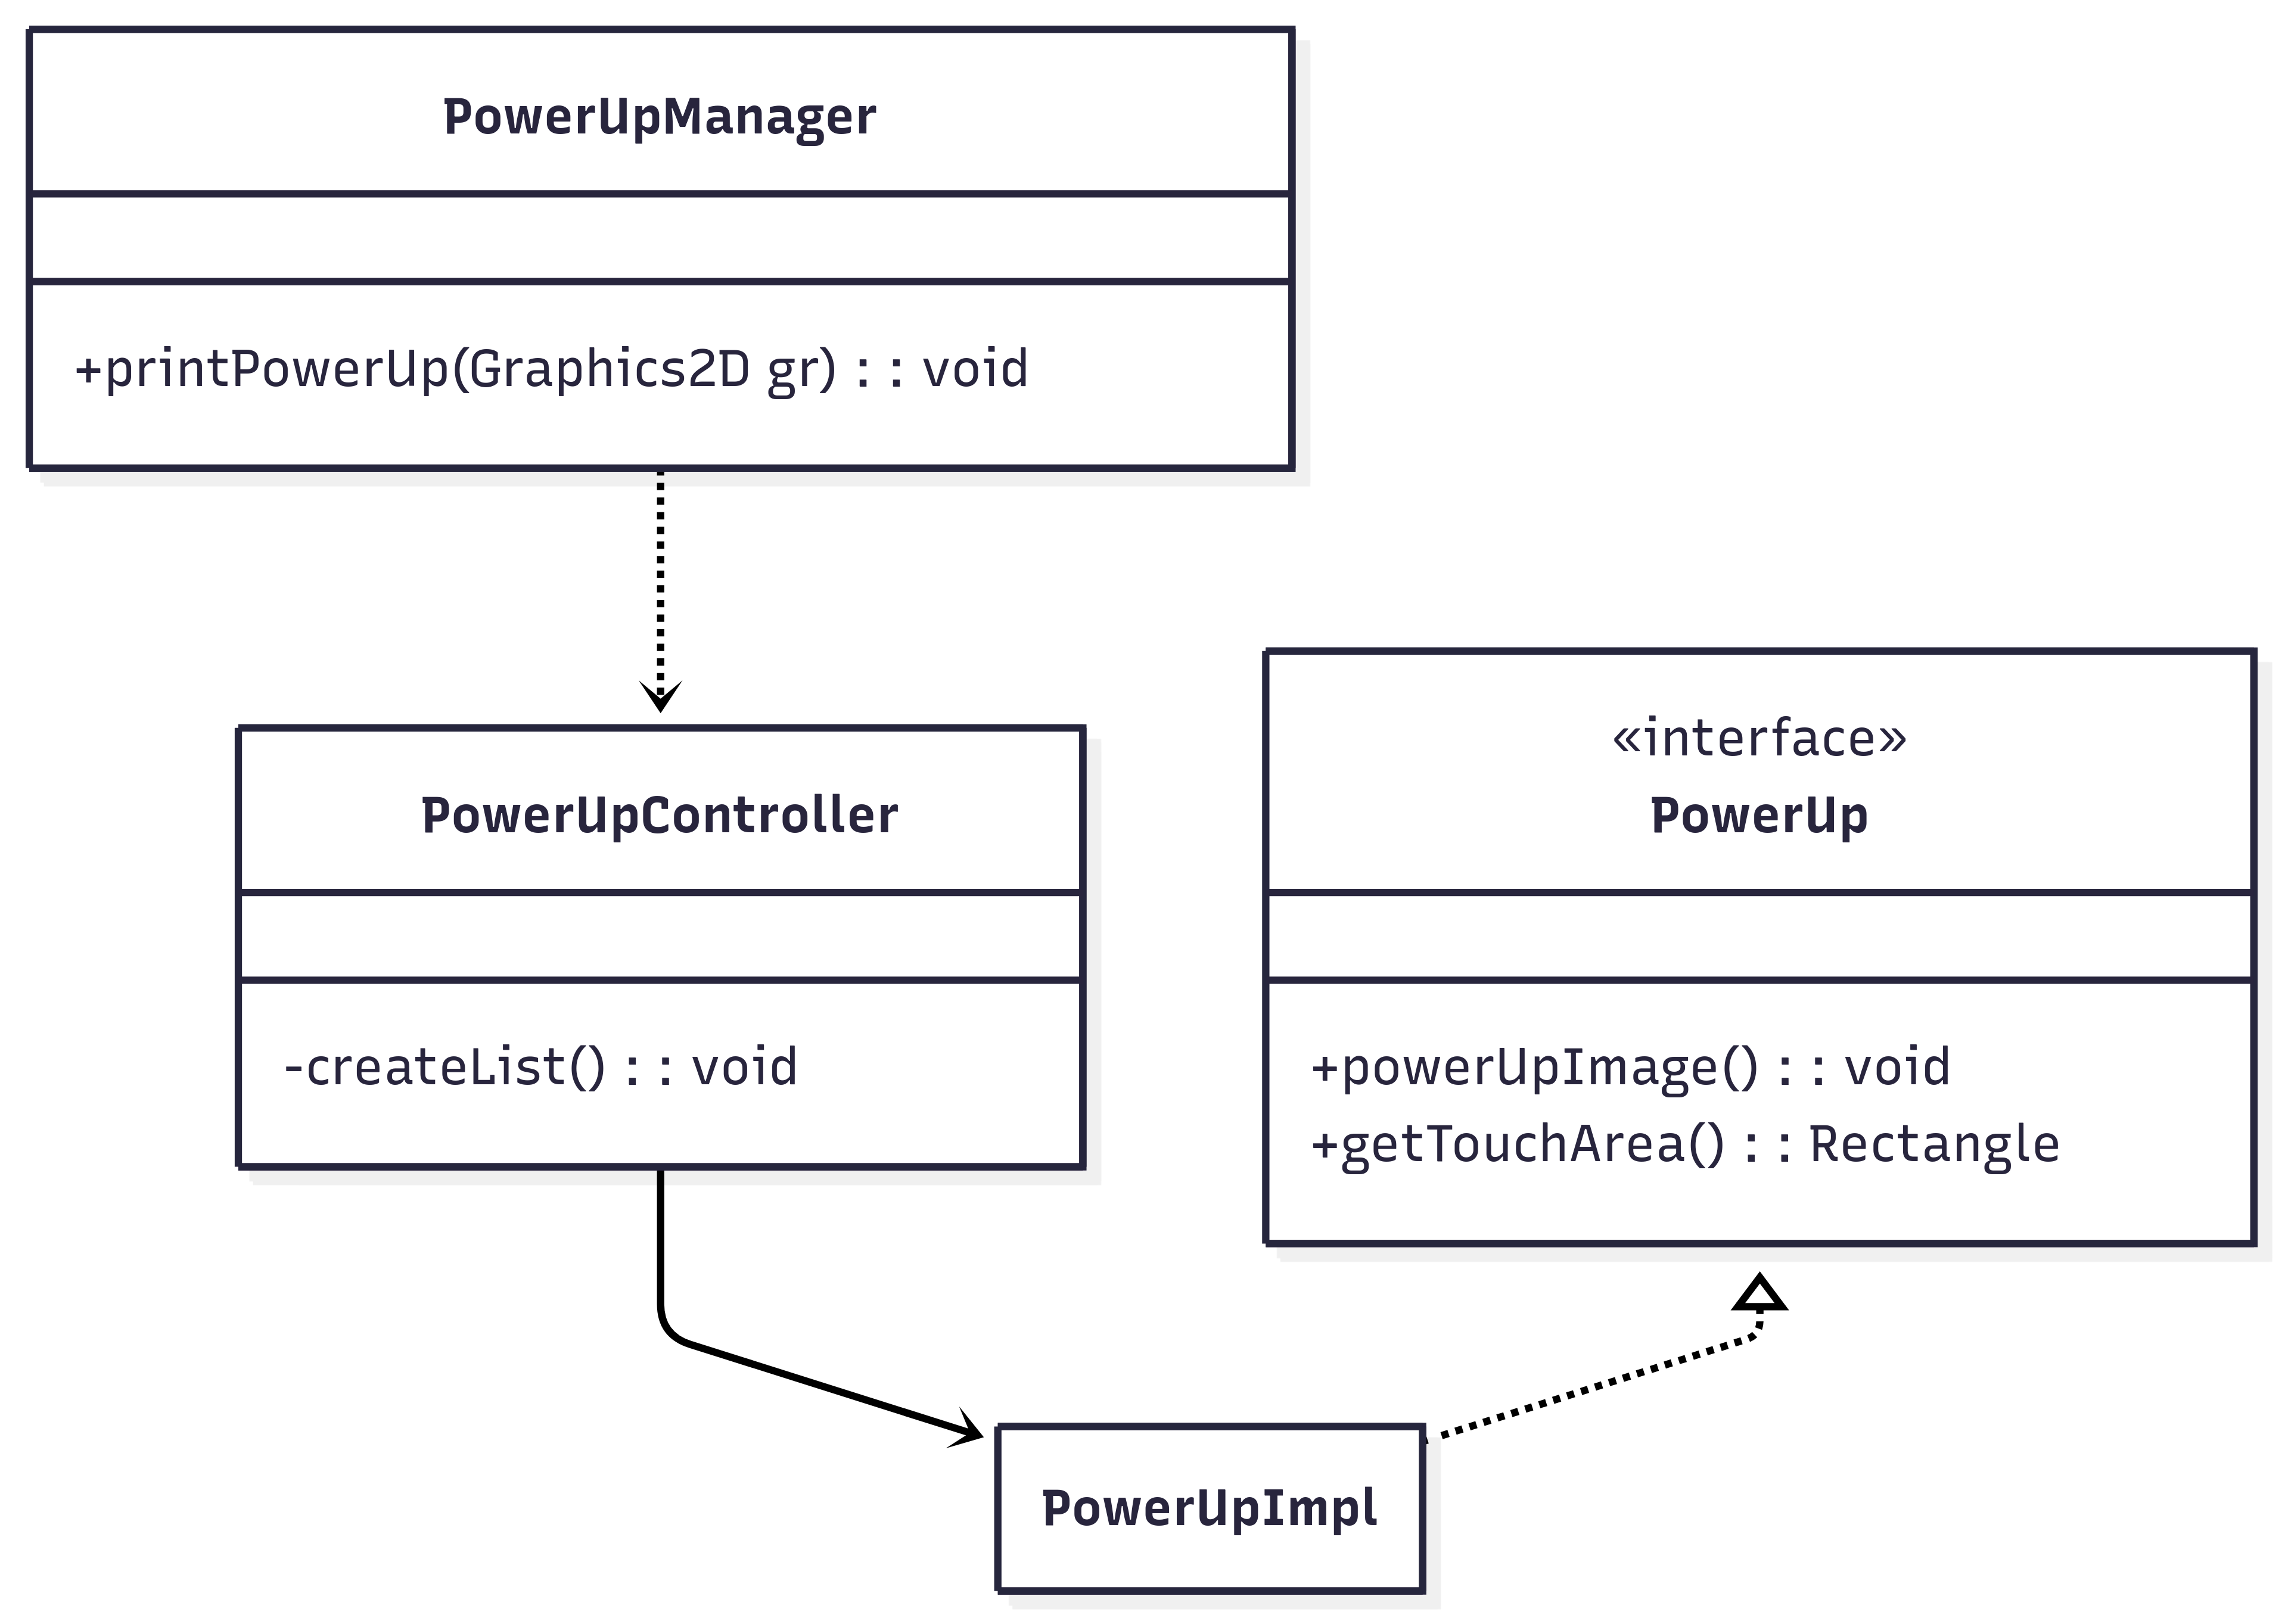
\includegraphics[width=0.8\textwidth]{resources/Powerup.png}
    \caption{UML architettura MVC dei powerup}
    \label{fig:2.4}
\end{figure}

\textbf{Problema}: gestire il passaggio da una skin all'altra in modo reattivo, in base alle diverse collisioni.\vspace{1cm}

\textbf{Soluzione}: creazione della classe PowersHandler nella sezione controller dell'MVC. La classe che gestisce l'inizializzazione del 
personaggio con cui si inzia il livello e la creazione di nuove istanze Character mantenendole in una lista. Quando il player ottiene 
1 vita (raccolta powerup) o la perde (collisione ostacolo o nemico, se non schiacciato) vengono utilizzati i metodi setPowers() e 
losePowers() dalle classi “Detection”; questi metodi si collegano al GameLoopController permettondo di cambiare la skin del player 
attualmente in gioco e di settare la posizione della nuova istanza all'interno della mappa. Inoltre permette di 
gestire il tempo in cui il player è immortale non appena perde una vita, tramite la variabile lastHit.
Infine fornisce il metodo gameOver() che restituisce true se l'entità Character è di tipo “Naked” e perde una vita.

\begin{figure}[H]
    \centering
    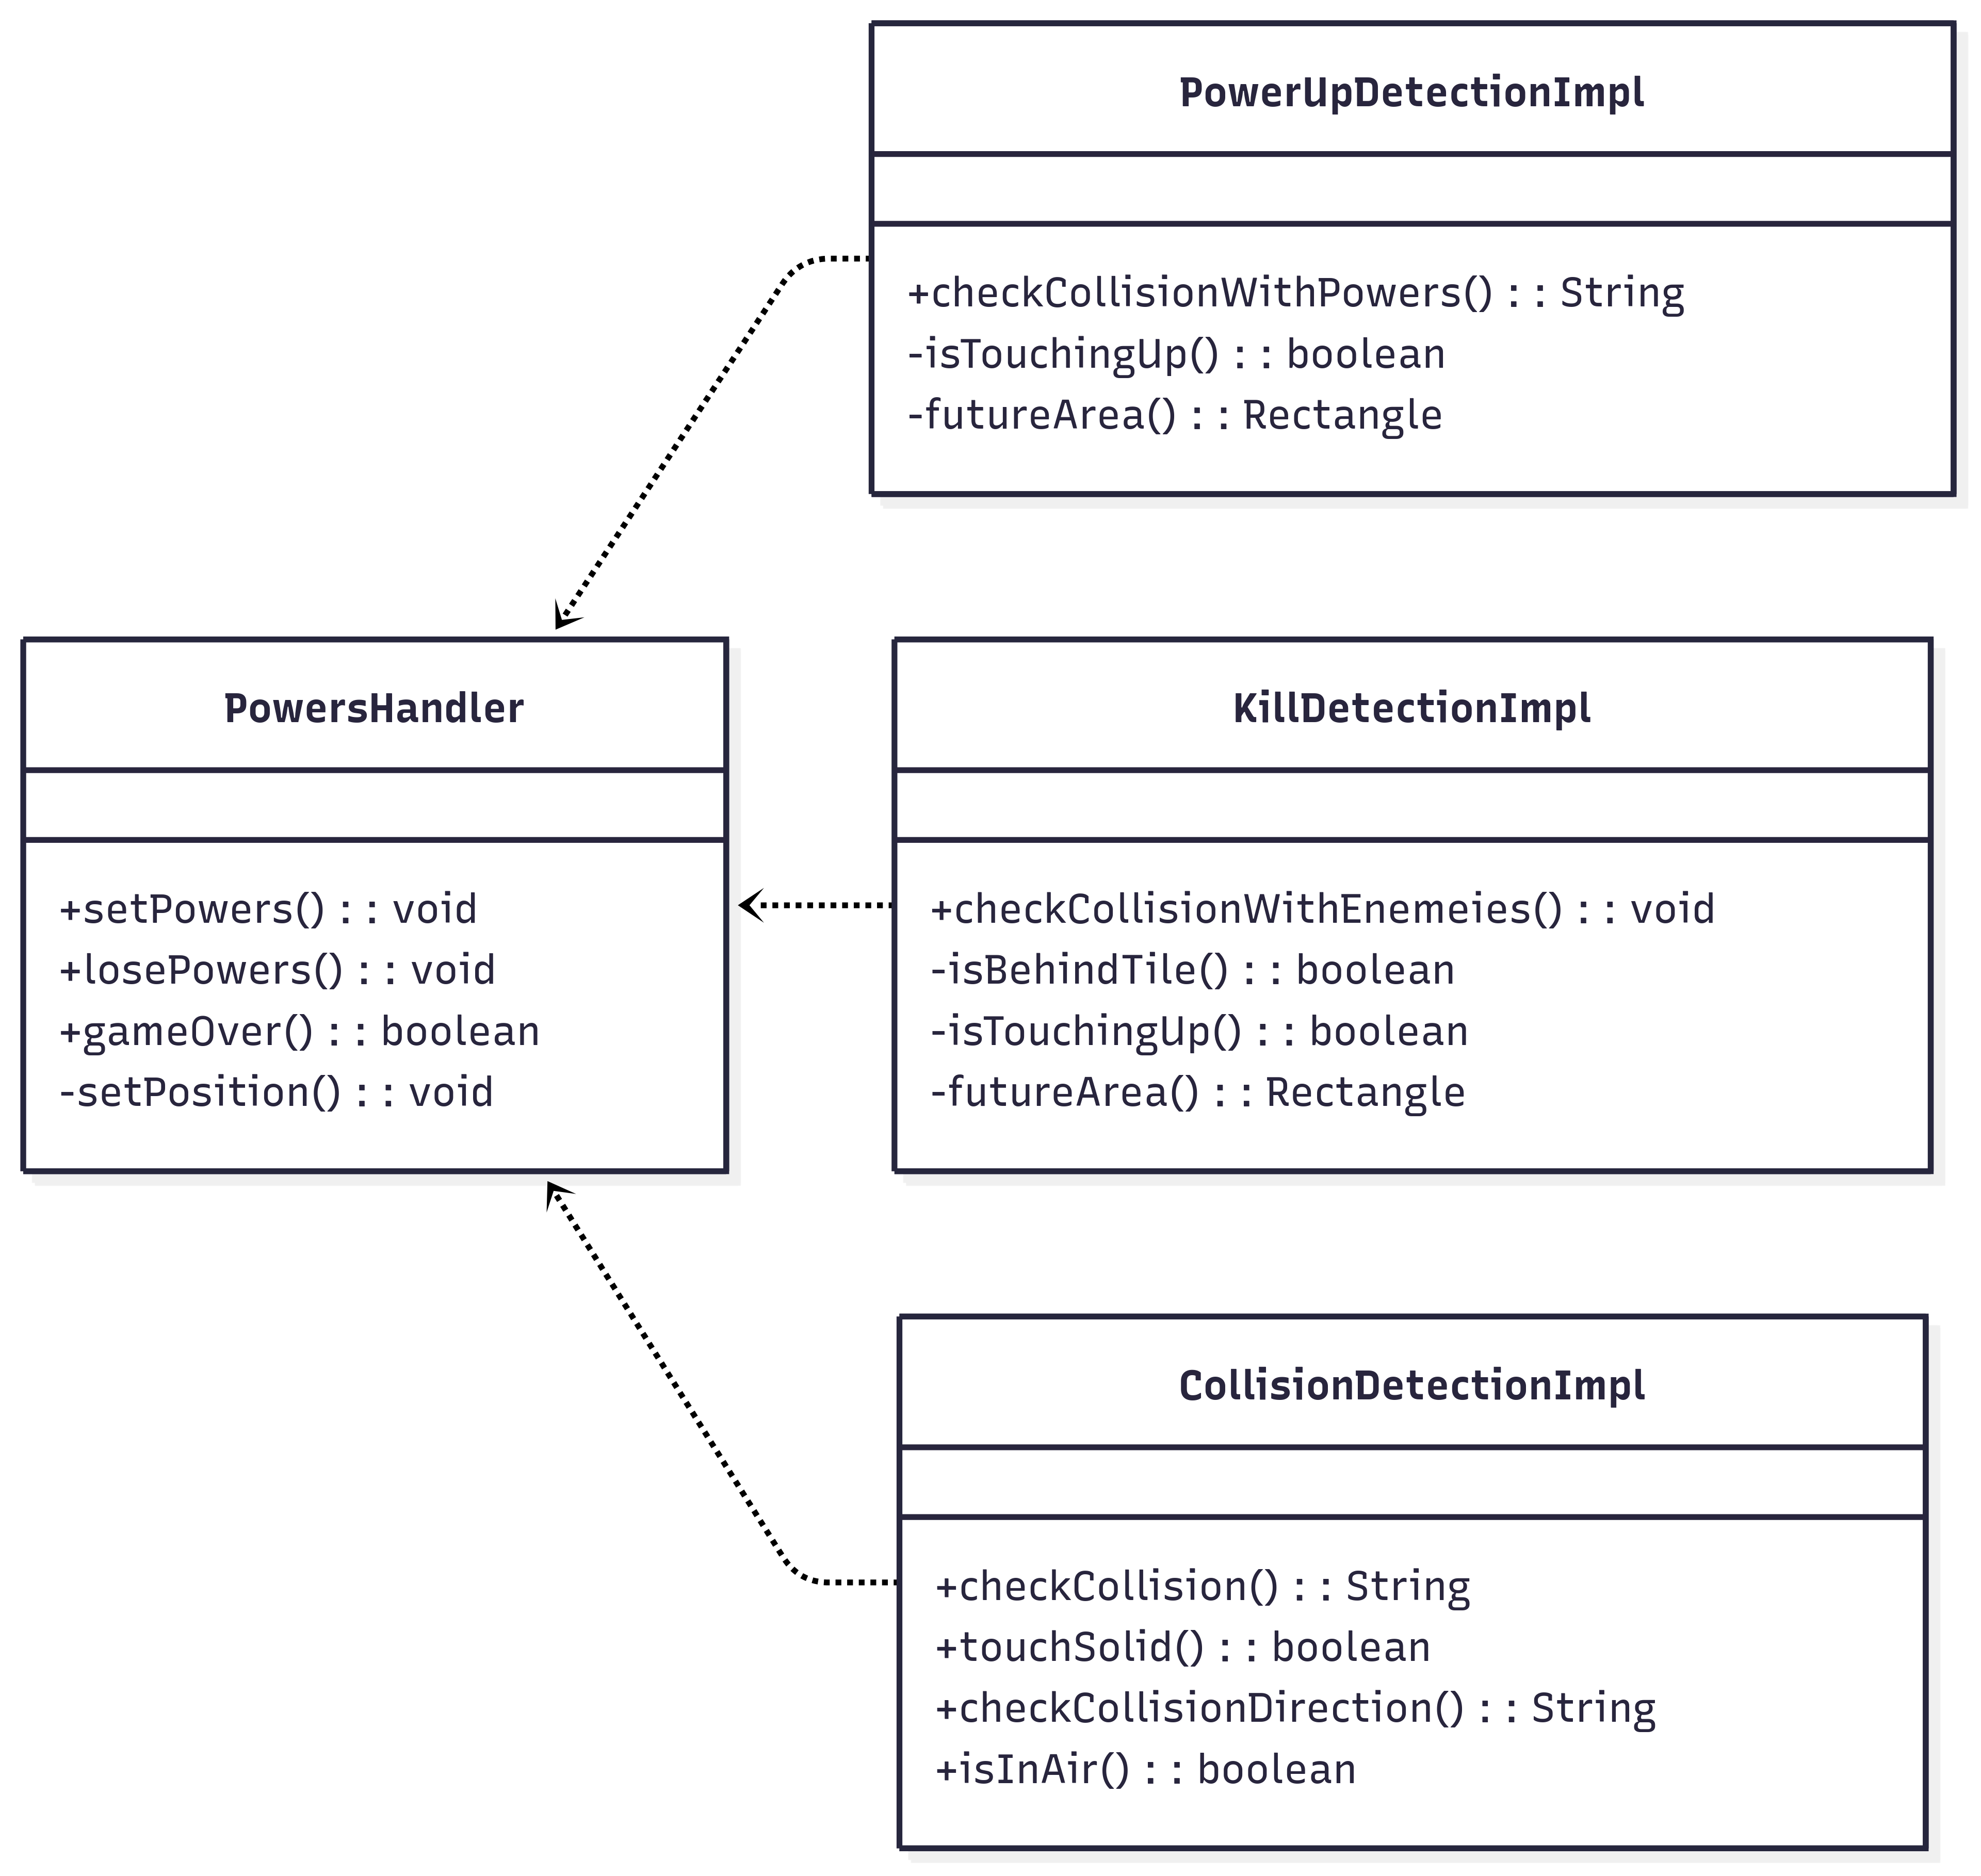
\includegraphics[width=0.8\textwidth]{resources/PowersHandler.png}
    \caption{UML architettura per gestire cambio skin in base alle collisioni}
    \label{fig:2.5}
\end{figure}

\section{Francesca Gatti}
\textbf{Problema}: Nel gioco è previsto un sistema di personalizzazione del personaggio tramite l'acquisto e la selezione di una nuova skin.
ALl'interno dello shop deve essere possibile selezionare a proprio piacimento la skin con cui si vuole iniziare a giocare. Infatti l'obiettivo dello
shop, oltre all'acquisto di una nuova skin, è quello di poter selezionare o la skin di default di gioco (\emph{Warrior}) o, una volta acquistata, una skin 
nuova (\emph{Wizard}). 
Il problema principale affrontato è stato quello di separare la gestione della parte logica del negozio, ovvero il controllo delle monete, 
delle skin e la selezione, dalla sua interfaccia grafica, mantenendo la possibilità di modificarlo in futuro.
\textbf{Soluzione}: Per affrontare questo problema è stato adottato il pattern \emph{Model-View-Controller} (MVC), suddividendo le responsabilità 
tra i tre livelli:
\begin{itemize}
    \item Model: rappresentato dalla classe \emph{Shop}, gestisce le skin disponibili, quella selezionata e lo stato di sblocco della skin (\emph{unlock}). 
    Nel model sono inoltre presenti le due classi \emph{Skin} e \emph{Score} che permettono la gestione degli oggetti skin e punteggio da parte dello Shop.
    \item View: la classe \emph{ShopView} è responsabile della visualizzazione delle informazioni (monete, stato skin) e della gestione dei pulsanti 
    che consentono l'acquisto e la selezione della nuova skin. L'utente è messo al corrente delle azioni che può fare nello shop grazie a 
    messaggi che appaiono una volta cliccato il pulsante desiderato.
    \item Controller: ho implementato l'interfaccia \emph{ShopController} che è responsabile della logica legata all'acquisto e alla selezione 
    delle skin e all'acquisizione dei dati e delle informazioni richieste dalla View. Inizialmente avevo implementato un'unica classe 
    all'interno del Model (la classe \emph{Shop}), ma il codice risultava molto pesante e difficile da gestire.
\end{itemize}
L'introduzione del pattern MVC ha permesso di ottenere una struttura più chiara, estendibile e orientata al riuso.
\begin{figure}
    \centering
    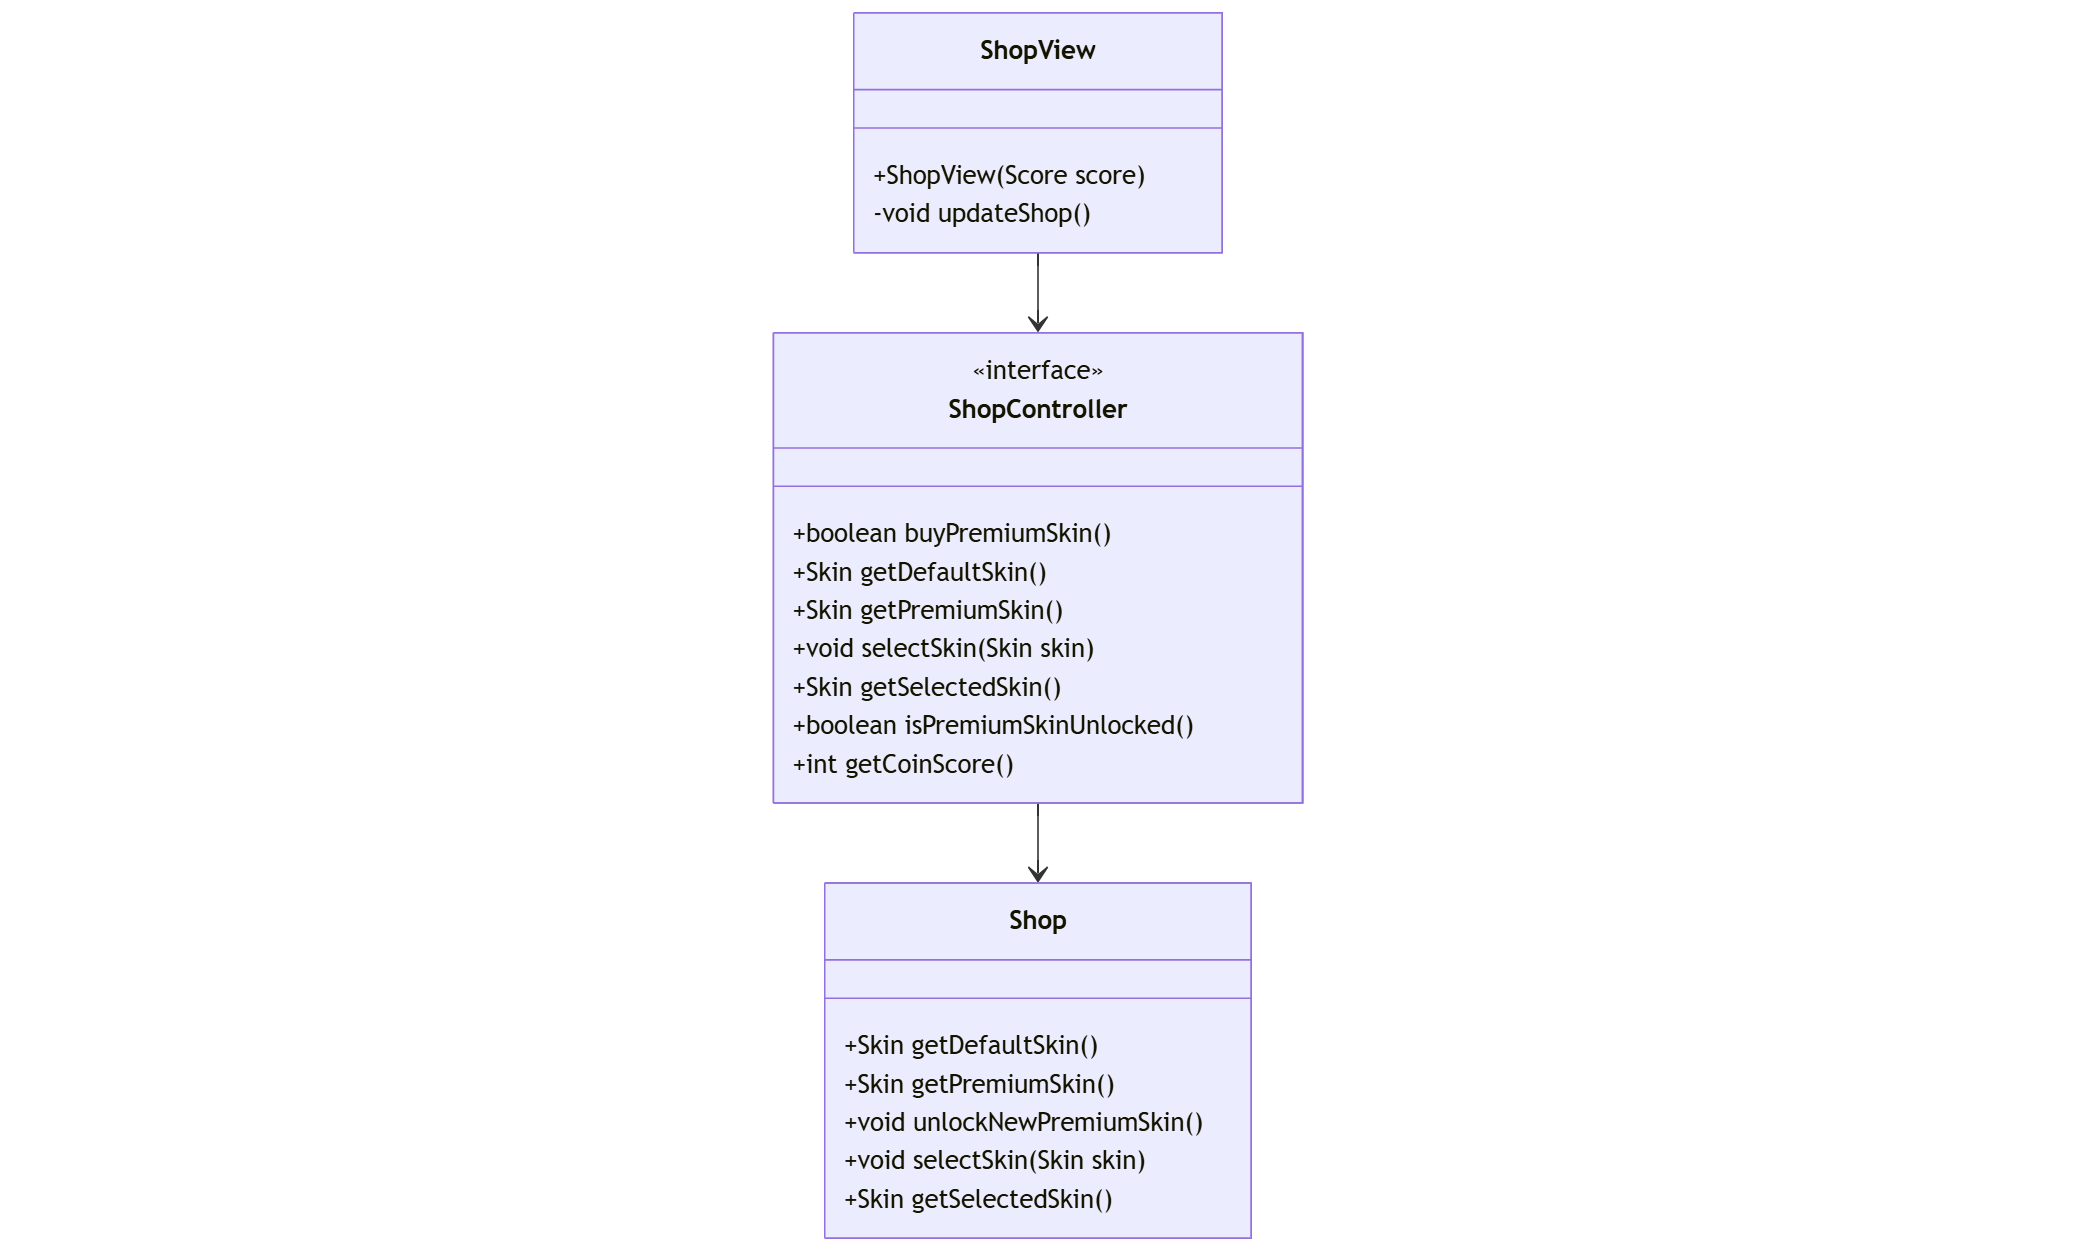
\includegraphics[width=0.8\textwidth]{resources/UMLshop.png}
    \caption{UML dell'MVC per la gestione dello shop}
    \label{fig: 2.2}
\end{figure}
\newpage
\textbf{Problema:} per lo sviluppo del gioco è stato necessario creare un sistema che gestisse la visualizzazione e la raccolta delle monete.
Le diverse funzionalità implementate sono il caricamento da file, il disegno delle monete sulla mappa, il rilevamento delle collisioni e 
l'aggiornamento di un punteggio.

\textbf{Soluzione:} ho creato questo sistema facendo una separazione logica delle responsabilità, suddividendo il sistema in più componenti
specializzate:
\begin{itemize}
    \item La classe \emph{Coin} rappresenta l'oggetto moneta, con le informazioni sulla posizione, il suo stato di raccolta e l'immagine.
    \item L'interfaccia \emph{CoinController} (impelementata da \emph{CoinControllerImpl}) gestisce il caricamento delle monete, la logica di 
    visualizzazione e il conteggio.
    \item L'interfaccia \emph{CoinDetection} (implementata da \emph{CoinDetectionImpl}) che si occupa del rilevamento delle collisioni tra player 
    e moneta.
\end{itemize}
Le classi sono collegate a \emph{Score}, \emph{ScoreController} e \emph{GameSaveManager} per il salvataggio del punteggio totale.
All'interno del \emph{CoinController} è stato necessario aggungere il metodo \emph{updatePlayer()} che permette l'aggiornamento delle monete 
in base ai cambiamenti subiti dal player durante il gioco, quali i potenziamenti. Senza la chiamata a questo metodo nel \emph{GameLoopController}, 
una volta acquisito il potenziamento da parte del player le monete non si caricavano più correttamente rimanendo fisse sullo schermo e non era più
possibile raccoglierle.

\textbf{Problema:} nel gioco era necessario monitorare il tempo di gioco trascorso, per poterlo visualizzare durante la partita e avere un 
resoconto finale del tempo impiegato per completare il livello.

\textbf{Soluzione:} Per affrontare il problema è stata creata l'interfaccia Chronometer che si occupa della gestione del tempo tramite un 
oggetto di tipo \emph{javax.swing.Timer}. Il timer aggiorna periodicamente il tempo trascorso in millisecondi rispetto al momento di avvio. La
classe fornisce metodi per avviare, fermare e ottenere il tempo in formato numerico e in formato stringa \emph{(HH::mm::ss::d)}. Infine, il tempo 
viene disegnato a schermo tramite la classe \emph{GameLoopPanel}, nel metodo \emph{paintComponent()}, che recupera il valore dal Chronometer e lo 
mostra in tempo reale durante il gioco.

\textbf{Problema:} è stato necessario implementare un sistema che permettesse di gestire il punteggio in base alle monete raccolte dal giocatore, con 
la possibilità di salvare questi dati in modo persistente o meno su scelta del giocatore. Questo sistema doveva inoltre integrarsi con altre parti del 
progetto, tra cui lo shop.

\textbf{Soluzione:} per gestire il punteggio ho sviluppato due componenti principali, basandomi sulla classe \emph{GameSaveManager}, ovvero un sistema di
salvataggio su file esterno. Le due componenti sono:
\begin{itemize}
    \item La classe \emph{Score} è il modello per la gestione delle monete raccolte. Al suo interno si trovano metodi per l'acquisizione del numero di monete
    salvate, per spenderle e, se necessario aggiungerne.
    \item L'interfaccia \emph{ScoreController} (implementata da \emph{ScoreControllerImpl}) ha il compito di aggiornare lo stato del punteggio nel file facendo 
    uso della classe \emph{GameSaveManager} come già detto sopra.
\end{itemize}

\section{Giovanni Maria Rava}
\textbf{Problema:} I nemici del gioco devono muoversi da soli, invertire direzione appena urtano un ostacolo e restare sincronizzati con 
lo scorrimento della camera. 

\textbf{Soluzione:} Per gestire il movimento autonomo e l'inversione di marcia in presenza di ostacoli ho adottato 
il pattern \emph{Model‑View‑Controller}. Il controller centrale è l'\emph{EnemyHandler}, che a ogni ciclo di gioco scorre l'intera lista di 
nemici: per ciascuno aggiorna prima lo stato logico delegando questa responsabilità all'oggetto model, \emph{EnemyImpl}, poi ne richiede 
la rappresentazione grafica all'oggetto view specifico, (ad esempio \emph{GoblinView}), per farla disegnare sul pannello di gioco. In questo modo 
la logica di collisione con la mappa e la scelta del momento in cui invertire la direzione restano incapsulate nel model, 
mentre il caricamento e il rendering rimangono confinati nella view; il controller non conosce i dettagli interni di nessuna delle due parti, 
ma si limita a coordinarne l'interazione. 
Questo assetto garantisce un codice più estendibile e manutenibile: introdurre una nuova tipologia di nemico richiede soltanto 
di aggiungere una nuova View, senza toccare il controller, e ogni modifica grafica o comportamentale resta circoscritta al relativo livello dell'architettura.~\ref{fig:2.9}
\begin{figure}
    \centering
    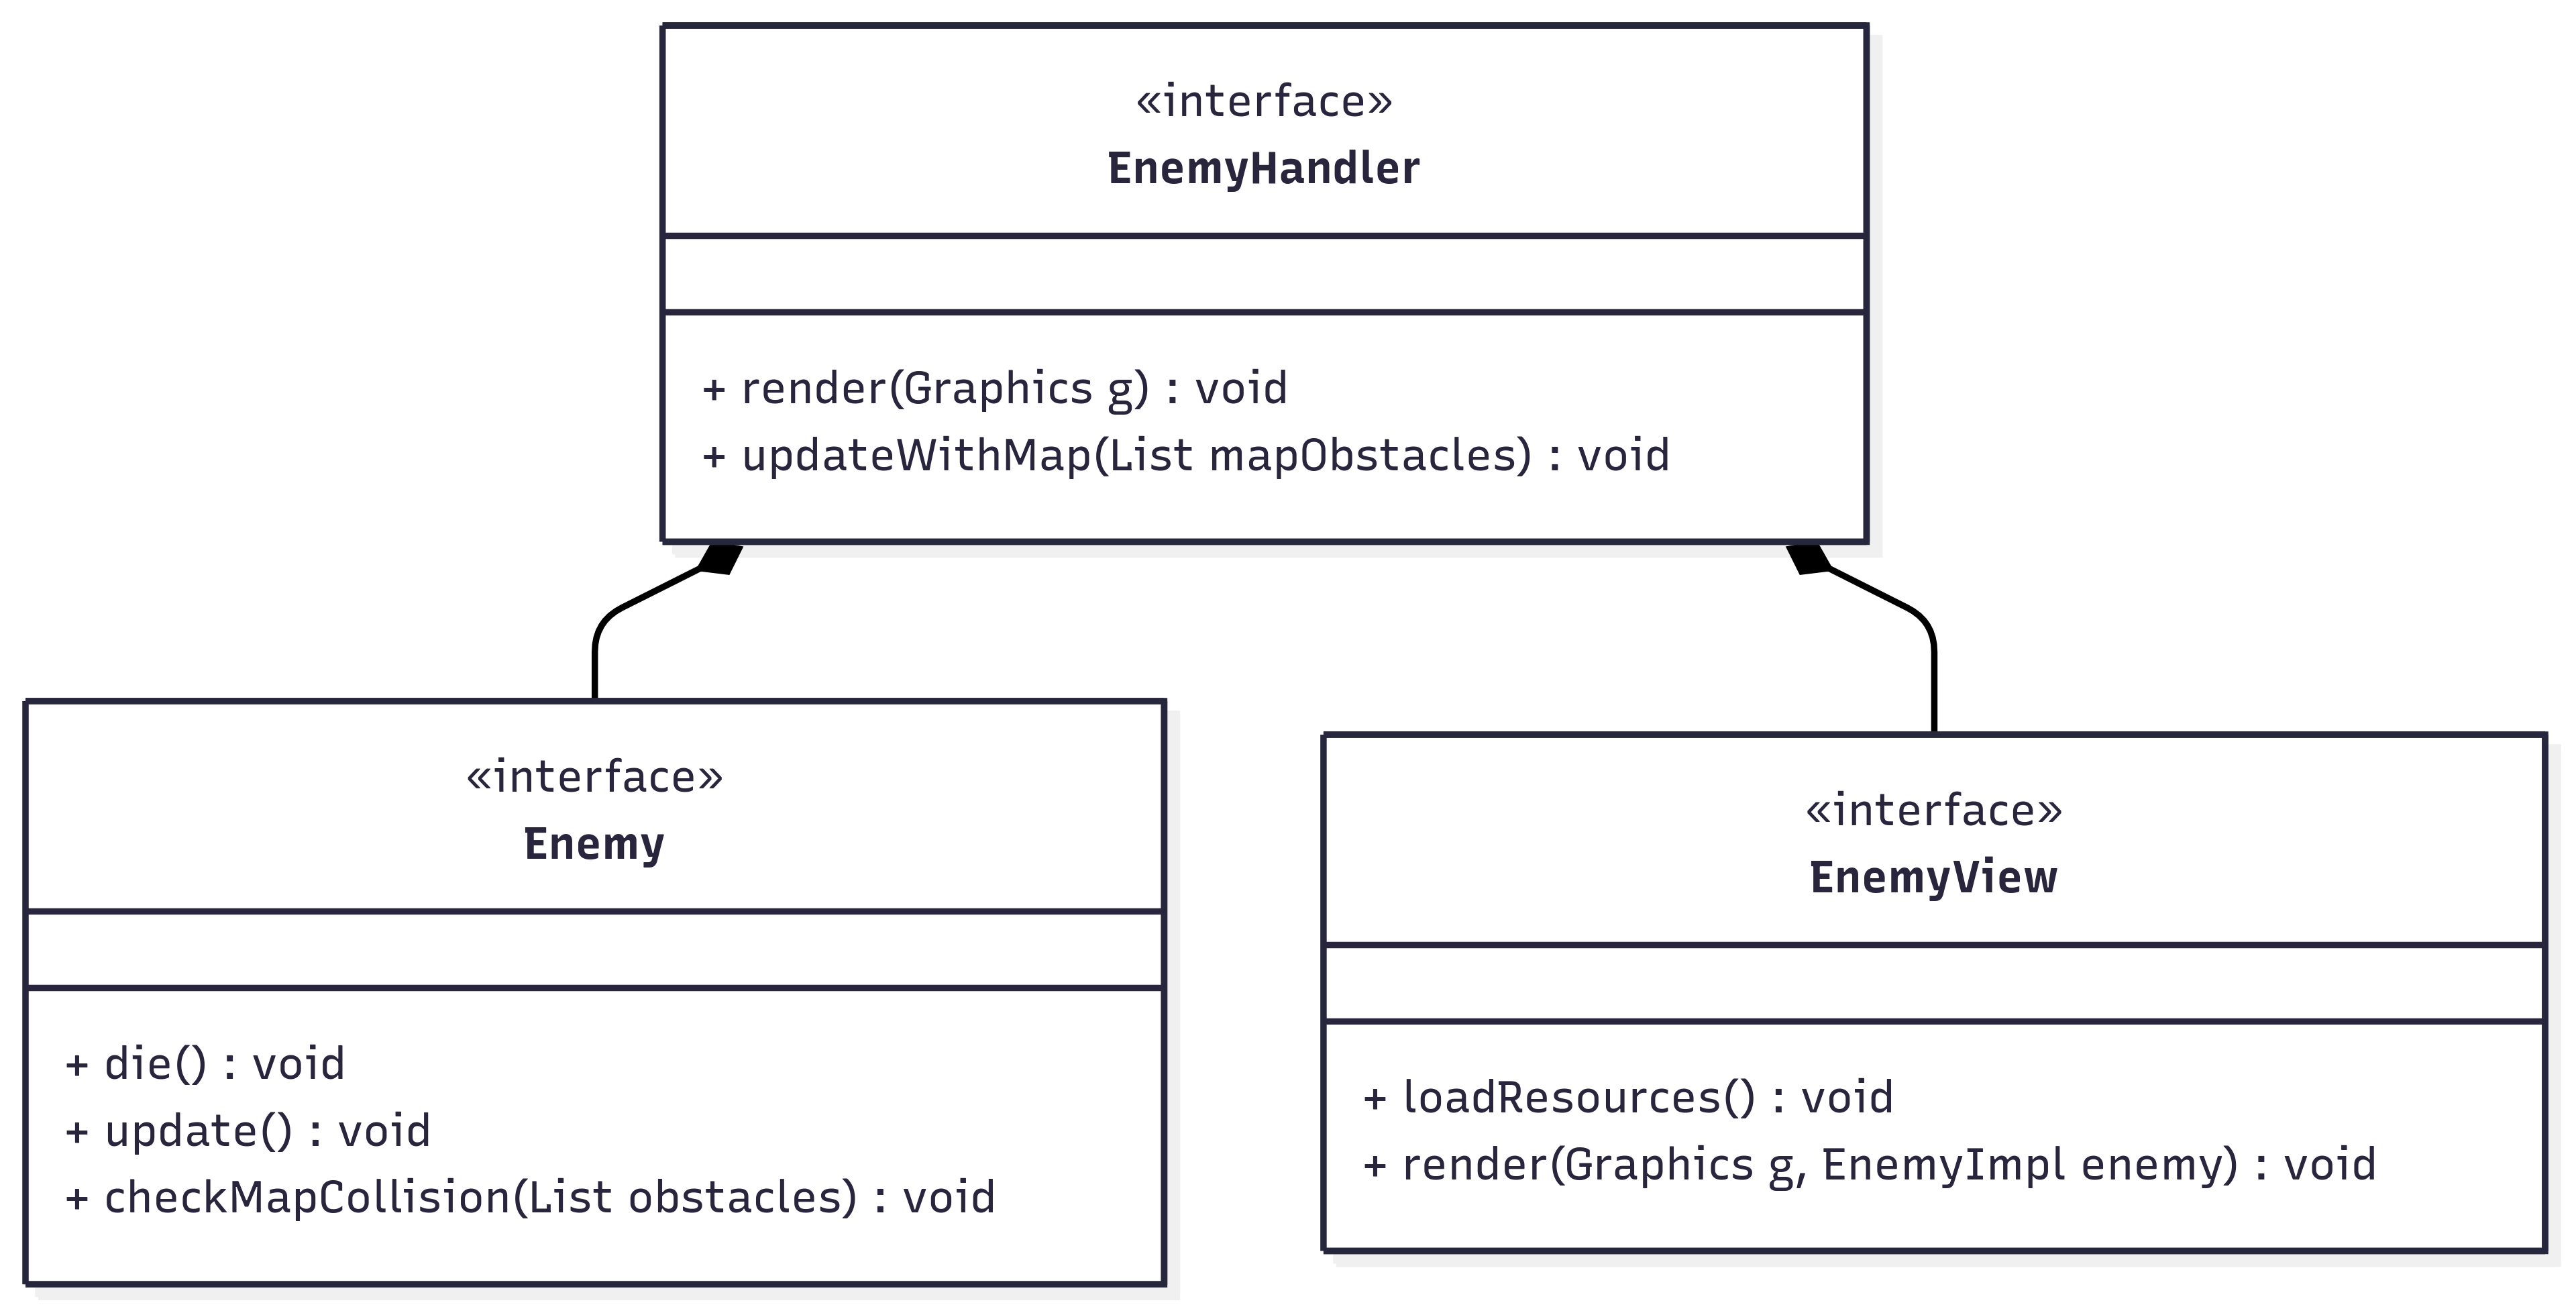
\includegraphics[width=0.8\textwidth]{resources/enemyMvcUml.png}
    \caption{UML dell'MVC per la gestione dei nemici}
    \label{fig:2.9}
\end{figure}
\newpage
\textbf{Problema:} Gestione il salvataggio del gioco e del caricamento del salvataggio all'apertura del gioco.\\
\textbf{Soluzione:} Il salvataggio e il ripristino della partita sono gestiti da un'unica classe, GameSaveManager, implementata 
come singleton tramite il pattern Initialization-on-demand holder idiom, una tecnica che garantisce accesso centralizzato, 
inizializzazione lazy e sicurezza thread-safe senza costi di sincronizzazione esplicita. \footnote{Questa implementazione è stata
 adottata per risolvere un warning PMD, come indicato in~\cite{pmd-singleton}, seguendo le linee guida descritte in~\cite{wiki-holder}.}

All'interno della classe, il caricamento dello stato avviene una sola volta al primo accesso all'istanza, tramite una classe interna statica (Holder) che 
richiama un metodo privato di inizializzazione. Questa logica garantisce che il file di salvataggio venga caricato una sola volta e 
che non vengano mai create più istanze del file, evitando duplicazioni o corruzioni dello stato.

Quando il giocatore completa un livello o chiude l’applicazione, i controller — in particolare ScoreController e CoinController — invocano i metodi pubblici del GameSaveManager 
per aggiornare lo stato di gioco, che comprende:
\begin{itemize}
    \item Un intero che indica i livelli completati.
    \item Un intero che indica le monete raccolte.
    \item Un booleano che indica l'acquisto della skin secondaria.
    \item Una stringa che indica la skin scelta.
\end{itemize}
All'avvio successivo, lo stato viene ricostruito e propagato ai vari model che lo necessitano; in caso contrario viene generata una partita nuova con parametri standard. 
L'intera logica di I/O è dunque isolata in una sola classe, priva di dipendenze dal motore di gioco; Questa architettura rende effettivo
il singleton e semplifica i test automatizzati.~\ref{fig:2.10}
\begin{figure}
    \centering
    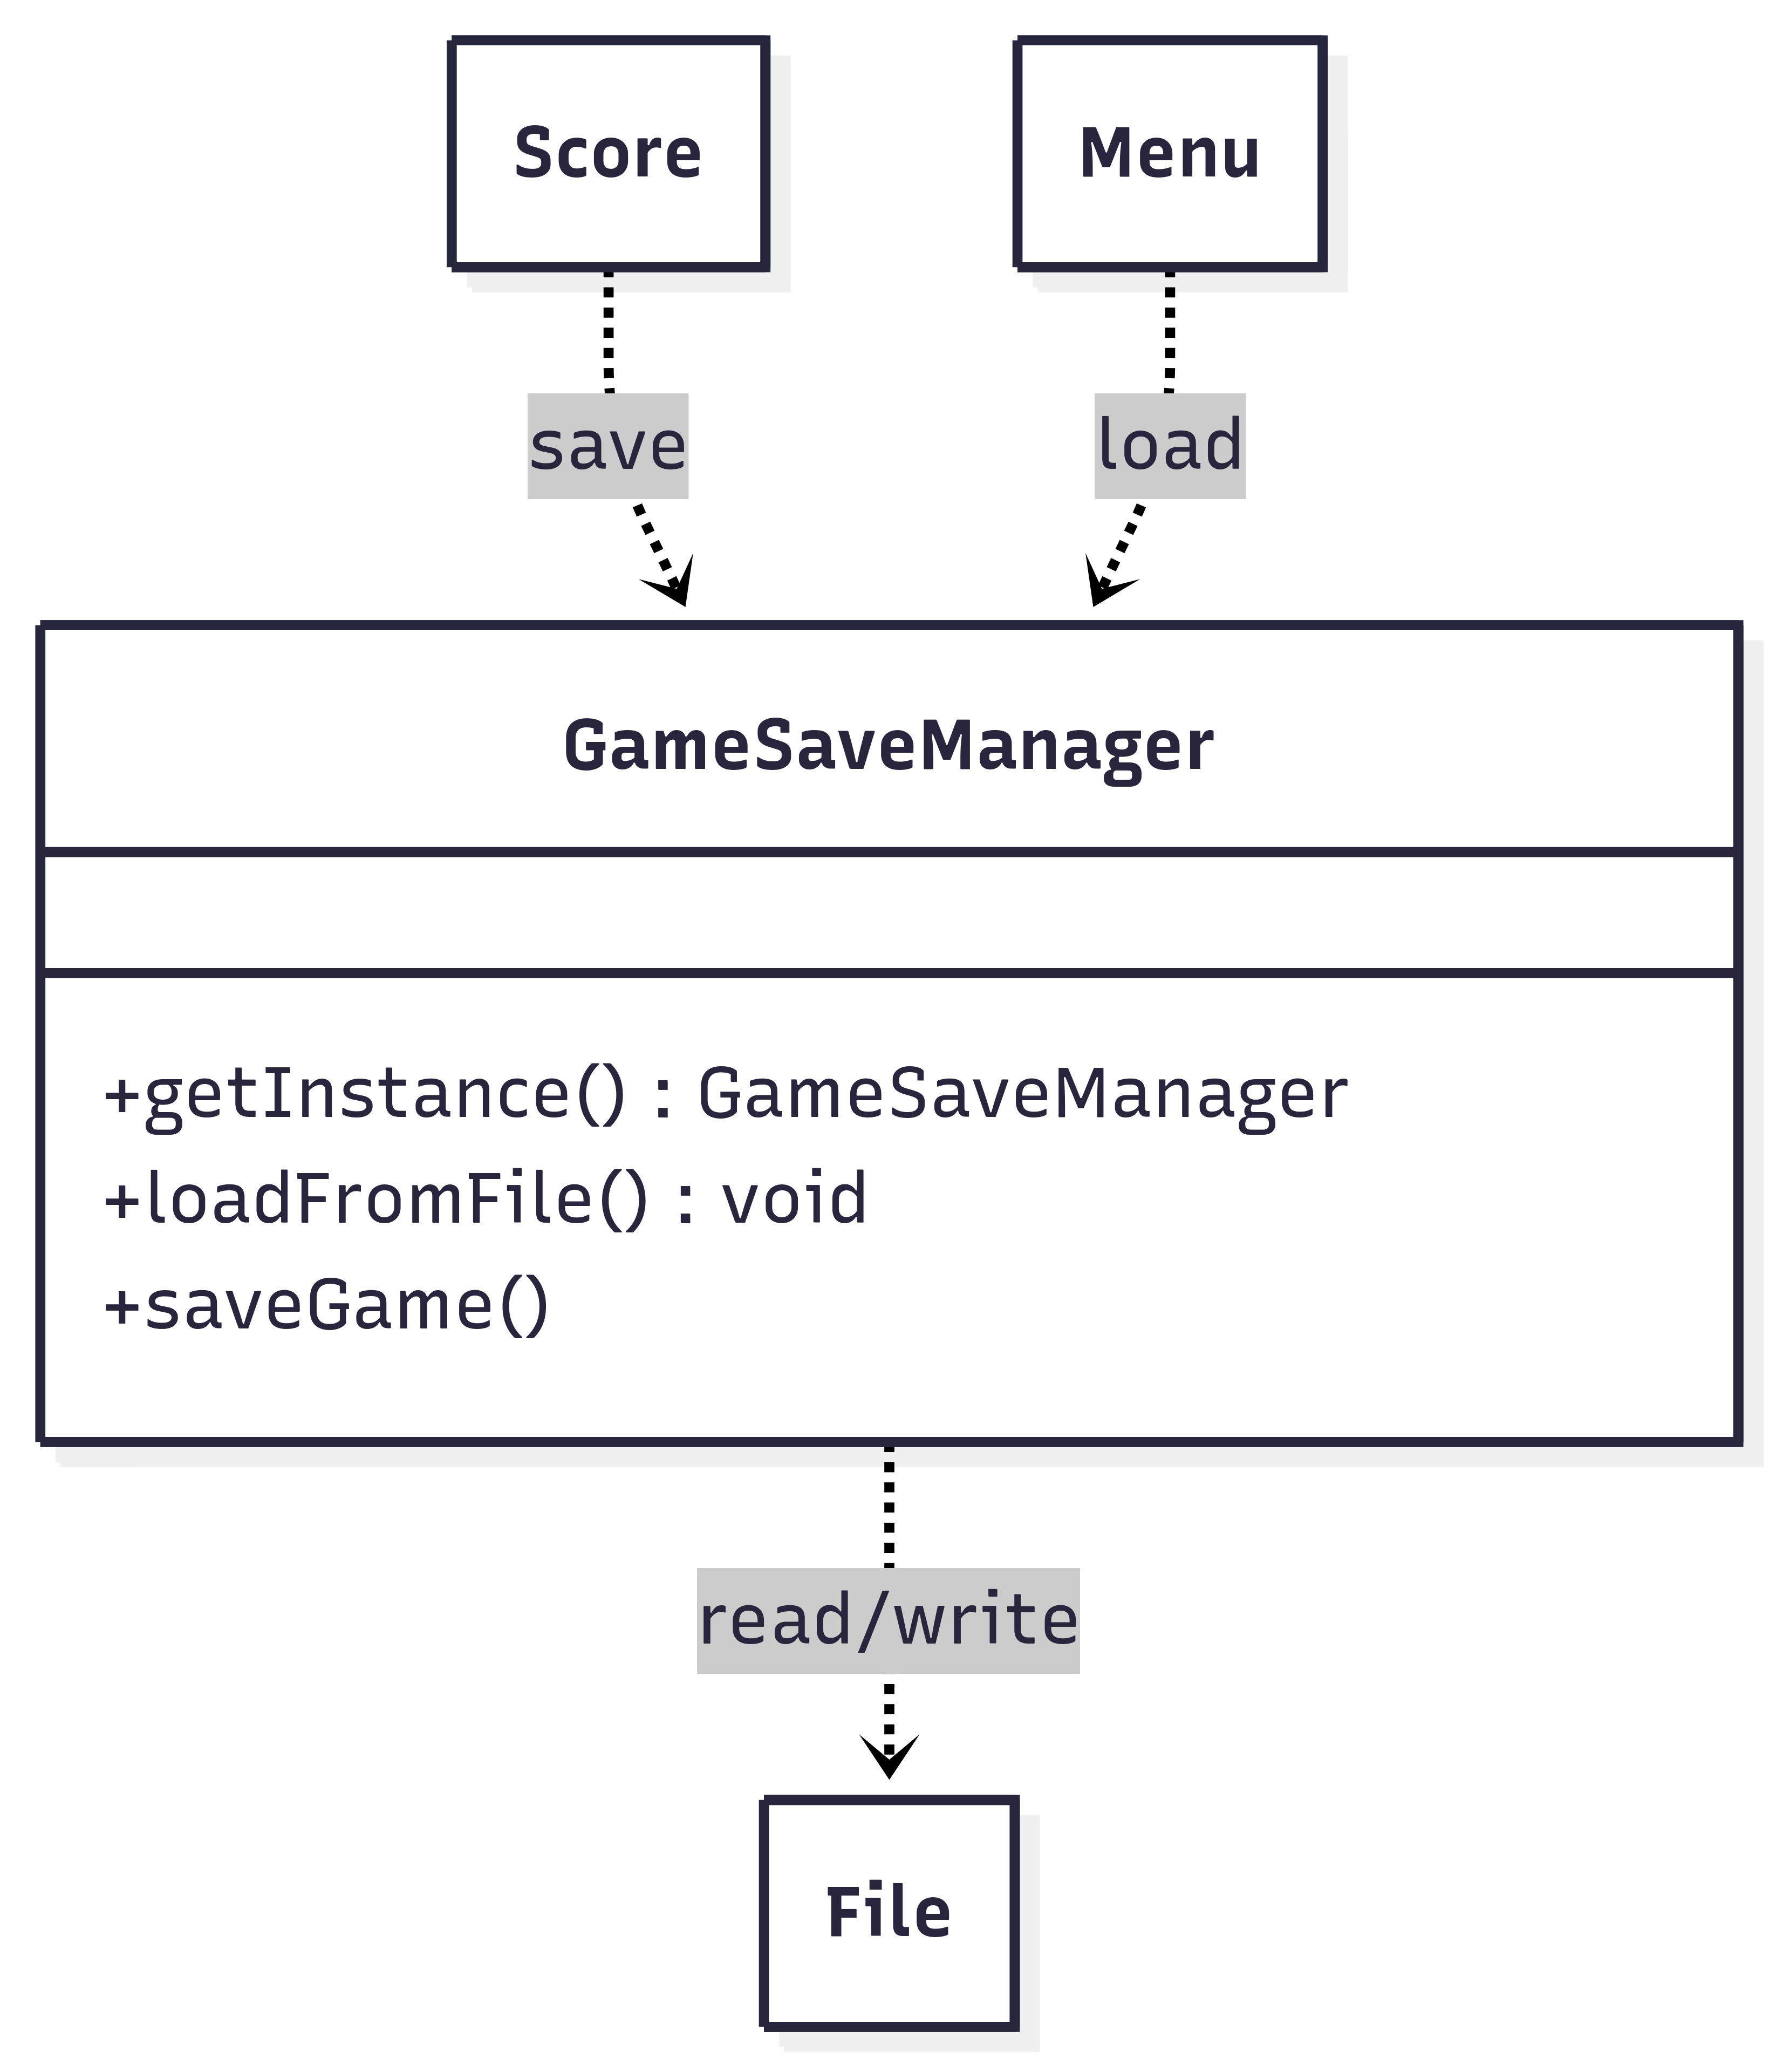
\includegraphics[width=0.6\textwidth]{resources/saveManagerUML.png}
    \caption{UML dell'MVC per la gestione dei nemici}
    \label{fig:2.10}
\end{figure}
\newpage
\textbf{Problema} Nel livello di gioco occorre generare molti nemici in posizioni predefinite: ognuno deve comparire al momento giusto,
nella coordinata corretta e con la propria grafica, ma senza mescolare la logica di lettura dei dati con la scelta delle view. 

\textbf{Soluzione:} Il file \emph{enemies*.txt}, letto da EnemySpawner, elenca riga per riga tipo di nemico e coordinate. 
Ogni riga viene trasformata in un oggetto immutabile EnemySpawnPoints, che serve come contenitore dei dati di spawn. Durante 
l'esecuzione EnemySpawner rimane in ascolto dello scorrimento della mappa di gioco: quando un punto di spawn entra nell'area visibile, 
istanzia il relativo modello di nemico e, anziché occuparsi direttamente della grafica, delega la creazione della vista a EnemyViewFactory. 
Quest'ultima contiene un metodo che riceve l'identificativo numerico del nemico e restituisce la classe di rendering adeguata; 
la sua implementazione concreta, EnemyViewFactoryImpl, contiene la mappatura fra tipologia e view corrispondente (as esempio 1 $\rightarrow$ GuardView).
In questo modo la lettura del file, la gestione della memoria e il caricamento delle immagini restano ben separati: per aggiungere un 
nuovo tipo di nemico è sufficiente aggiungere una riga al file di mappa e una voce nella factory, senza toccare né il game‑loop né lo 
spawner, mantenendo il sistema estendibile e pulito.~\ref{fig:2.11}
\begin{figure}
    \centering
    \includegraphics*[width=0.8\textwidth]{resources/spawingEnemyUML.png}
    \caption{UML gestione spawing nemici}
    \label{fig:2.11}
\end{figure}
\chapter{Sviluppo}
\section{Testing automatizzato}
I test sono stati scritti con JUnit 5, quindi Gradle li esegue automaticamente e l'intera suite gira senza alcun intervento manuale.
Ogni caso di prova carica risorse dedicate, in particolare mappe di test, copie ridotte e semplificate di quelle di produzione, così
l'esito non risente di eventuali modifiche ai livelli reali. La combinazione fra esecuzione automatizzata e risorse isolate garantisce 
che l'intero motore grafico, la gestione dei nemici e la correttezza del sistema di salvataggio vengano controllati con rapidità, 
senza interferenze con il materiale definitivo del gioco.

Per quanto riguarda i nemici, i test verificano la corretta restituzione del proprio Rectangle, assicurano che le collisioni con gli
altri elementi della mappa siano gestite a dovere, e controllano l'inversione della velocità in caso di impatto con un ostacolo.
Con la medesima logica, la classe TestGoblinView verifica il caricamento corretto delle immagini.

GameSaveManagerTest accerta che il pattern singleton sia rispettato, impedendo la creazione di più istanze del gestore dei 
salvataggi. Controlla il corretto funzionamento della scrittura e lettura tramite file.

Il test riguardante il player è TestPlayerCollision, che ha lo scopo di verificare con 4 test le possibili interazioni del player con
le altre entità. Si è settata uan dimensione di default dei blocchi della mappa.
Quindi vengono verificati i metodi principali delle classi "Detection". Nel caso dei blocchi di mappa e delle uova,
vengono verificate le direzioni delle collisioni. Si verifica poi se il player raccoglie in modo corretto il powerup e se cambia skin.
Il cambio di skin viene verificato anche quando il player collide con un nemico; se la collisione avviene dall'alto il nemico 
invece muore. Infine si verifica se le monete vengono raccolte.

Il ChronometerTest verifica il corretto funzionamento della classe ChronometerImpl (che implementa l'interfaccia Chronometer) per la
gestione del Timer di gioco. Il test assicura che il cronometro misuri correttamente il tempo trascorso e che la sua rappresentazione 
testuale (che poi nel gioco si visualizza a schermo) sia corretta. In test fallisce nel caso in cui il tempo non venga misurato 
correttamente o nel caso di una formattazione errata.

Il CoinTest verifica il corretto funzionamento del caricamento delle coordinate, dell'inizializzazione degli oggetti Coin e la gestione 
dello stato di raccolta: la moneta non deve risultare raccolta prima della chiamata a collect(). Il test è importante per garantire l'affidabilità 
del caricamento e del disegno delle monete sulla mappa di gioco.


\section{Note di sviluppo}
\section{Samuele Bianchedi}
Una delle scelte di design più importanti del progetto è stata la rigorosa applicazione dei principi di incapsulamento e immutabilità.
L’analisi iniziale con SpotBugs ha rivelato criticità rispetto all’esposizione interna. 
Queste ultime erano potenziali bug difficilmente riconoscibili, in quanto i dati erano vulnerabili a modifiche esterne non controllate.
Si è adottata la tecnica delle copie difensive in questi seguenti modi:
\begin{itemize}
    \item Robustezza: il design incapsulato rende il software meno vulnerabile a bug di side effect, 
    perché lo stato degli oggetti è protetto e controllato.
    \item Manutenibilità: separando la parte pubblica e privata di una classe contribuisce a facilitare la correzione 
    o l’aggiunta di parti di codice senza “rompere” altre parti del programma.
    \item Portabilità: L’uso di UTF-8 in modo esplicito garantisce lo stesso comportamento su piattaforme diverse.
\end{itemize}
Tra le feature avanzate troviamo:
\begin{itemize}
    \item Uso di Generics: per garantire la type safety nelle collezioni, come Map<Integer, BufferedImage> e List<MapElement>
    https://github.com/GiovanniRava/OOP24-runwarrior/blob/59f5771e783f0430bcbb4859ef986df97121394a/src/main/java/it/unibo/runwarrior/model/GameMap.java
    \item API di I/O: utilizzo di java.nio.charset.StandardCharset per spcificare l’encoding UTF-8 in lettura
https://github.com/GiovanniRava/OOP24-runwarrior/blob/59f5771e783f0430bcbb4859ef986df97121394a/src/main/java/it/unibo/runwarrior/model/MapLoader.java
\end {itemize}

\section{Riccardo Cornacchia}
\begin{itemize}
    \item Implementazione della classe \textbf{KeyListener} mediante CharacterComand per ricevere input da tastiera. $\rightarrow$ Permalink:
    \url{https://github.com/GiovanniRava/OOP24-runwarrior/blob/786d60909eb4856d26449dafa053fcec146400df/src/main/java/it/unibo/runwarrior/controller/player/CharacterComand.java#L9}
    \item Implementazione della classe \textbf{GameMusic} mediante nuovi tipi AudioInputStream, AudioSystem e Clip. 
    Utilizzata per musica in background ed effetti sonori. $\rightarrow$ Permalink:
    \url{https://github.com/GiovanniRava/OOP24-runwarrior/blob/786d60909eb4856d26449dafa053fcec146400df/src/main/java/it/unibo/runwarrior/view/GameMusic.java#L17}
    
    Per questa implementazione ho fatto riferimento al seguente sito $\rightarrow$
    \url{https://www3.ntu.edu.sg/home/ehchua/programming/java/J8c_PlayingSound.html}
    \item Uso di \textbf{stream e lambda expression} nella classe CollisionDetectionImpl. Mi permette di organizzare gerarchicamente 
    le diverse direzioni di collisione in cui è coinvolto il player. $\rightarrow$ Permalink:
    \url{https://github.com/GiovanniRava/OOP24-runwarrior/blob/786d60909eb4856d26449dafa053fcec146400df/src/main/java/it/unibo/runwarrior/controller/collisions/impl/CollisionDetectionImpl.java#L74}
\end{itemize}

\section{Francesca Gatti}
\begin{itemize}
    \item \textbf{Utilizzo lambda expression} $\rightarrow$ Permalink:
    \url{https://github.com/GiovanniRava/OOP24-runwarrior/blob/786d60909eb4856d26449dafa053fcec146400df/src/main/java/it/unibo/runwarrior/view/Menu.java#L181C17-L192C20}
    \url{https://github.com/GiovanniRava/OOP24-runwarrior/blob/786d60909eb4856d26449dafa053fcec146400df/src/main/java/it/unibo/runwarrior/view/Menu.java#L193C17-L204C20}
    \url{https://github.com/GiovanniRava/OOP24-runwarrior/blob/786d60909eb4856d26449dafa053fcec146400df/src/main/java/it/unibo/runwarrior/view/Menu.java#L205C16-L216C20}
    \url{https://github.com/GiovanniRava/OOP24-runwarrior/blob/1177dc7188d3a96ba1165ba19e439a1417d417bf/src/main/java/it/unibo/runwarrior/view/Menu.java#L226C17-L235C20}
    \item
\end{itemize}
\section{Giovanni Maria Rava}
\begin{itemize}
    \item \textbf{Utilizzo di stream e lambda expression} $\rightarrow$ Permalink: 
    \url{https://github.com/GiovanniRava/OOP24-runwarrior/blob/487ae1a3598382a5eb6584d892bbe61fabc8d758/src/main/java/it/unibo/runwarrior/controller/enemy/EnemySpawner.java#L55-L63}
    \item \textbf{Utilizzo di lambda expressione} $\rightarrow$ Permalink:
    \url{https://github.com/GiovanniRava/OOP24-runwarrior/blob/487ae1a3598382a5eb6584d892bbe61fabc8d758/src/test/java/it/unibo/runwarrior/model/GameSaveManagerTest.java#L63}
    \item \textbf{Implementazione metodo copyImage} $\rightarrow$ Permalink:
    \url{https://github.com/GiovanniRava/OOP24-runwarrior/blob/ea221779e7801710824877e7599505de2931ca1d/src/main/java/it/unibo/runwarrior/view/enemy/impl/GoblinView.java#L91-L98}
    Per risolvere un warning PMD di tipo EI EXPOSE REP, che segnala l'esposizione diretta di oggetti mutabili, in questo caso un BufferedImage, è stato introdotto un metodo privato 
    che crea una copia sicura dell'immagine da restituire. In questo modo si evita che il chiamante possa modificare direttamente lo stato interno della classe, preservando l'incapsulamento.
    La copia viene realizzata tramite un nuovo BufferedImage su cui si disegna l'immagine originale usando un oggetto Graphics2D, 
    ottenuto con createGraphics(). Questo approccio è documentato nella pagina ufficiale Oracle della classe Graphics, sezione 
    create(...), vedi \cite{oracle-graphics-create}.
\end{itemize}

\chapter{Commenti finali}
\section{Autovalutazione e lavori futuri}
\subsection{Samuele Bianchedi}
Direi che non ci sono grandi punti di forza, il lavoro funziona e fa il suo dovere. Ho cercato di mantenere tutto semplice e comprensibile,
senza aggiungere funzioni complicate, creando classi che si occupano di un solo compito per volta.
Ho cercato di fare del mio meglio, tra impegni, lavoro e tutto il resto. Ogni tanto ho rotto il programma e i miei compagni mi hanno aiutato
a riparare i miei errori. Avrei potuto essere più attivo nel gruppo e apportare qualche contributo in più.
Sicuramente mi è piaciuto e mi ha divertito e mi ha spronato a impegnarmi di più in vista di futuri esami.

\subsection{Riccardo Cornacchia}
\textbf{Sviluppi futuri}: implementazione di nuove skin da inserire nel Template pattern, sia per i personaggi esistenti, sia per 
nuovi personaggi, creando nuove classi ed estendendo AbstractCharacterImpl.
In relazione a ciò appena detto si può aggiungere l'implementazione di nuovi powerups: aggiungerne dei nuovi ai personaggi esistenti o 
modificare quelli esistenti.
Implementazione di nuovi metodi da parte delle sottoclassi di AbstractCharacterImpl che possano definire nuove meccaniche di gioco, 
ad esempio: salto doppio, gestione di nuove azioni determinate da evntuali nuovi powerup, accovacciamento.

\textbf{Autovalutazione}: sin dall'inizio dello sviluppo del progetto, penso che mi sia focalizzato con serietà e dedizione su come 
realizzare la nostra idea e in particolar modo su come definire la mia parte, che ad oggi posso dire essere il frutto di una continua 
ricerca avvenuta mediante tante idee giuste e sbagliate.
Uno degli aspetti che mi ha tenuto maggiormente occupato e su cui ho speso un'importante parte del mio lavoro, è la realizzazione 
delle collisioni, in particolar modo le collisioni tra player e blocchi della mappa, da cui ho 
poi sviluppato anche le altre classi di gestione delle collisioni; per questo credo che questo aspetto sia un punto di forza della 
mia parte di codice.

Altro aspetto su cui ho lavorato tanto è stata la meccanica di movimento del player, che step by step è arrivata ad essere ciò che è 
ora, ma credo che in quel caso, una volta impostati gli input da tastiera, si potessero prendere diverse strade per svilupparla, 
giungendo alla stessa conclusione ma con un codice eventualmente migliore, o anche peggiore chissà, in confronto a quello da me sviluppato.
Cito anche la parte relativa ai potenziamenti e la classe PowersHandler che penso essere ben adeguate all'architettura MVC.

Complessivamente penso di essere riuscito ad avere un approccio attivo e stimolante con il gruppo di lavoro, con cui mi sono confrontato 
con continuità e grazie al quale siamo riusciti a risolvere diversi problemi in maniera più efficiente.

\subsection{Giovanni Maria Rava}
All'interno del progetto mi sono occupato principalmente di una parte che penso sia importante ma comunque non essenziale per il 
gioco ovvero i nemici. Ho avuto la difficoltà principale nella gestione della loro nascita, in quanto ho cercato di importare una 
modalità che potesse essere modificabile in un futuro senza però dover intaccare la parte di codice. Ho poi utilizzato il restante
tempo per lo sviluppo di un sistema di salvataggio del gioco, nel migliorare l'architettura delle mie parti e nel controllo degli 
spotbugs. La parte al quale ho sicuramente dato meno attenzione è quella di sviluppo della grafica. Gli sviluppi futuri di questa 
parte sono molti, tra i principali  ci sono: nuovi nemici e/o ostacoli, l'implementazione di un movimento più complesso dei nemici,
ad esempio quello verticale. In futuro potrebbe essere implementato uno spawning dinamico e una meccanica in cui, alla morte di un
nemico, venga generato un oggetto bonus o malus.
Il progetto è stato stimolante a livello personale ma sopratutto è stato un ottimo modo per migliorare la capacità di lavorare in 
gruppo. Il gruppo mi è stato molto di aiuto per superare le criticità incontrate e darci una mano quando le cose non andavano come 
volevamo.
\appendix
\chapter{Guida utente}
Per il movimento del player si usano 4 frecce della tastiera:
\begin{itemize}
    \item \textbf{Freccia destra}: per muoversi verso destra
    \item \textbf{Freccia sinistra}: per muoversi verso sinistra
    \item \textbf{Freccia in alto}: per saltare, più la si preme più il salto sarà alto.
    Mentre si è in volo il player si può muovere a destra e sinistra.
    \item \textbf{Shift}: per attaccare con spada o bastone nel caso in cui si è giunti al secondo potenziamento.
    Attenzione, mentre si è in movimento il player può attaccare una volta ogni secondo.
\end{itemize}
\chapter{Bibliografia}
\begin{thebibliography}{9}

    \bibitem{pmd-singleton}
    PMD Project,\\
    \emph{PMD Java Rule: NonThreadSafeSingleton},\\
    \url{https://docs.pmd-code.org/pmd-doc-7.12.0/pmd_rules_java_multithreading.html#nonthreadsafesingleton},\\
    accessed July 2025.
    
    \bibitem{wiki-holder}
    Wikipedia contributors,\\
    \emph{Initialization-on-demand holder idiom} --- Wikipedia,\\
    \url{https://en.wikipedia.org/wiki/Initialization-on-demand_holder_idiom},\\
    accessed July 2025.

    
    \bibitem{oracle-timer}
    Oracle Corporation,\\
    \emph{Timer (Java Platform SE 8)} --- Oracle Docs,\\
    \url{https://docs.oracle.com/javase/8/docs/api/java/util/Timer.html},\\
    accessed May 2025

    \bibitem{oracle-keylistener}
    Oracle Corporation,\\
    \emph{KeyListener (Java Platform SE 8)} --- Oracle Docs,\\
    \url{https://docs.oracle.com/javase/8/docs/api/java/awt/event/KeyListener.html},\\
    accessed April 2025

    \bibitem{chua-sound}
    Chua Hock-Chuan,\\
    \emph{Java: Playing Sound (Audio Clip, MP3, Java Sound API)} --- NTU Tutorials,\\
    \url{https://www3.ntu.edu.sg/home/ehchua/programming/java/J8c_PlayingSound.html},\\
    accessed May 2025

    \bibitem{oracle-graphics-create}
    Oracle,\\
    \emph{Graphics.create(int x, int y, int width, int height) Method Documentation},\\
    \url{https://docs.oracle.com/javase/8/docs/api/java/awt/Graphics.html#create-int-int-int-int-},\\
    accessed July 2025.

    \end{thebibliography}

\end{document}